%%%% IACR Transactions TEMPLATE %%%%
% This file shows how to use the iacrtrans class to write a paper.
% Written by Gaetan Leurent gaetan.leurent@inria.fr (2020)
% Public Domain (CC0)


%%%% 1. DOCUMENTCLASS %%%%
\documentclass[journal=tosc,preprint]{iacrtrans}
%%%% NOTES:
% - Change "journal=tosc" to "journal=tches" if needed
% - Change "submission" to "final" for final version
% - Add "spthm" for LNCS-like theorems


%%%% 2. PACKAGES %%%%
\usepackage{lipsum} % Example package -- can be removed
\usepackage{tikz} % For drawing the arrow
\usepackage{tcolorbox}
\usepackage{listings}
\usepackage{xcolor}
\usepackage{graphicx} % For including images
\usepackage{subcaption} % For subfigures and subcaptions


\usetikzlibrary{matrix, positioning}

\lstset{
    basicstyle=\ttfamily\footnotesize,
    keywordstyle=\bfseries\color{blue},
    frame=single, % Adds a border
    numbers=false, % Line numbers
    numberstyle=\tiny\color{gray},
    commentstyle=\color{green!60!black},
    stringstyle=\color{orange},
    showstringspaces=false,
    breaklines=true,
    backgroundcolor=\color{gray!10},
}

%%%% 3. AUTHOR, INSTITUTE %%%%
\author{Lalit Gour\inst{1,2} \and Vedant Udan\inst{1,3} \and Karan Sunil Kumbhar\inst{1,4}}
% \institute{
%   Indian Institute of Technology Bhilai, India, \email{lalitg@iitbhilai.ac.in}
%   \and
%   Indian Institute of Technology Bhilai, India, \email{udanvedant@iitbhilai.ac.in}
%   \and
%   Indian Institute of Technology Bhilai, India, \email{karansunilk@iitbhilai.ac.in}
% }

\newcommand{\iitbhilai}{Indian Institute of Technology Bhilai, India}

% \author{
%   Lalit Gour\inst{1} \and Vedant Udan\inst{1} \and Karan Sunil Kumbhar\inst{1}
% }
\institute{
  \iitbhilai \and \email{lalitg@iitbhilai.ac.in} \and
  \email{udanvedant@iitbhilai.ac.in} \and
  \email{karansunilk@iitbhilai.ac.in} 
}


%%%% NOTES:
% - We need a city name for indexation purpose, even if it is redundant
%   (eg: University of Atlantis, Atlantis, Atlantis)
% - \inst{} can be omitted if there is a single institute,
%   or exactly one institute per author


%%%% 4. TITLE %%%%
\title{Midori - Implementation and Analysis}
%%%% NOTES:
% - If the title is too long, or includes special macro, please
%   provide a "running title" as optional argument: \title[Short]{Long}
% - You can provide an optional subtitle with \subtitle.

\begin{document}

\maketitle


%%%% 5. KEYWORDS %%%%
\keywords{Midori64 \and DDT/LAT analysis \and Integral Cryptanalysis \and Differential Crytanalysis \and MILP Model}


%%%% 6. ABSTRACT %%%%
\begin{abstract}

    In this paper we discuss the algorithm to implement Midori Cipher perform
    Integral and Differential Cryptanalysis on it.

\end{abstract}


%%%% 7. PAPER CONTENT %%%%
\section{Introduction}

The Midori cipher, introduced by Banik et al. in 2015, is a lightweight block
cipher specifically designed for resource-constrained environments such as IoT
devices and embedded systems. It emphasizes energy efficiency and low power
consumption while ensuring robust security against standard cryptographic
attacks. Midori comes in two variants: Midori-64 (64-bit block size, 128-bit
key) and Midori-128 (128-bit block size, 128-bit key), both based on a
Substitution-Permutation Network (SPN) structure. By employing simple operations
like XOR, substitution (S-box), and diffusion via MixColumn, Midori achieves
high energy efficiency and compact hardware implementation, making it
well-suited for applications in smart cards, wearables, and RFID systems. While
its lightweight design balances security and performance, its reduced complexity
compared to heavyweight ciphers like AES may make it vulnerable to advanced
attack scenarios.

\section{Integral Cryptanalysis}
Similar to Differential but here we use a Set of Plaintexts known as Delta Set (\(\Delta\)) instead of just two.
\subsection{Basic Knowledge }
\subsubsection{Definition of Integral Property}
\begin{itemize}
    \item \textbf{Constant \( \mathcal{C} \)}: The constant byte is constant whose value is fixed and unchanged.
    \item \textbf{Active \( \mathcal{A} \)}: Bytes traverse all values of 0 - 15, which is called active byte.
    \item \textbf{Balance \( \mathcal{B} \)}: The sum of bytes is 0, which is called balanced byte.
    \item \textbf{Unknown \( \mathcal{U} \)}: If the nature of a byte is uncertain, it is called an unknown byte.
\end{itemize}
The linear combination of active bytes \( \mathcal{A} \) and constant
bytes \( \mathcal{C} \) is active byte \( \mathcal{A} \). The constant bytes \( \mathcal{C} \) and
balance bytes \( \mathcal{B} \) are balance \( \mathcal{B} \) after the linear operation.
Independent active bytes \( \mathcal{A} \) is active \( \mathcal{A} \) after linear
combination. The linear combination of two related active \( \mathcal{A} \)
is balance \( \mathcal{B} \). Balance \( \mathcal{B} \) changes into unknown \( \mathcal{U} \) through
nonlinear bijection. Active \( \mathcal{A} \) has the characteristics of
penetration to S-box and AddRoundKey. And so on.
\subsubsection{Delta Set (\(\Delta\)) }
\begin{itemize}
    \item We will be taking a Set of 16 Plaintexts called Delta Set (\(\Delta\)) where 4 bits of each plaintext takes all values from \( \{0, 1\}^4 \) and the rest of the 60 bits have constant values.
    \item In case of Midori64 Bit Block we get the following:
          \[
              P_0 = (0, c_1, c_2, \dots, c_{14}, c_{15}),
          \]
          \[
              P_1 = (1, c_1, c_2, \dots, c_{14}, c_{15}),
          \]
          \[
              \vdots
          \]
          \[
              P_{15} = (15, c_1, c_2, \dots, c_{14}, c_{15}),
          \]

          and the Delta Set (\( \Delta \)) is defined as:

          \[
              \Delta = \{P_0, P_1, \dots, P_{15}\}.
          \]

    \item The Initial Plaintext Set (\(\Delta\)) in terms of \( \mathcal{A} \), \( \mathcal{C} \) and \( \mathcal{B} \).

          \[
              \Delta = \{\( \mathcal{A} \), \( \mathcal{C} \),\( \mathcal{C} \), \dots, \( \mathcal{C} \)\}.
          \]

\end{itemize}
\subsubsection{Symbol}

The meaning of the symbolic representation below:

\begin{align*}
    s_j^{(i)} & : \text{The } j\text{-th byte of the } i\text{-th round input.}      \\
    m_j^{(0)} & : \text{The } j\text{-th byte of the plaintext.}                     \\
    c_j^{(i)} & : \text{The } j\text{-th byte in the } i\text{-th round ciphertext.} \\
    k_j^{(i)} & : \text{The } j\text{-th byte in the } i\text{-th round key.}        \\
    R_i       & : \text{The } i\text{-th round.}
\end{align*}


\subsection{Description of Midori}
Midori is a lightweight block ciphers which follows the
Substitution-Permutation Network (SPN) design approach.
The grouping of the Midori algorithm expressed by State
Matrix and Each element in the matrix is a Cell. The State
Matrix is a 4 × 4 matrix, as shown in Fig. 1. For the two
algorithms which have different packet length, each Cell
contains different vector lengths. The length of each Cell of
the Midori64 is 4-bit. The length of each Cell of the
Midori128 is 8-bit. And the unified definition of the left end
of each Cell vector is MSB, the right end of each Cell vector
is LSB.



\[
    \begin{bmatrix}
        S_{0} & S_{4} & S_{8}  & S_{12} \\
        S_{1} & S_{5} & S_{9}  & S_{13} \\
        S_{2} & S_{6} & S_{10} & S_{14} \\
        S_{3} & S_{7} & S_{11} & S_{15}
    \end{bmatrix}
\]

\begin{center}
    Fig.1 : State matrix of midori.
\end{center}

\subsubsection{SubCell (\( \mathcal{S} \))}

The S-box type of Midori used by 4-bit S-box. The 4-bit
S-boxes is shown in TABLE I. The S-boxes of Midori64 correspond to ${S_0(x)}

    \begin{table}[h!]
        \centering
        \begin{tabular}{|c|c|c|c|c|c|c|c|c|c|c|c|c|c|c|c|c|}
            \hline
            x          & 0 & 1 & 2 & 3 & 4 & 5 & 6 & 7 & 8 & 9 & a & b & c & d & e & f \\ \hline
            ${S_0(x)}$ & c & a & d & 3 & e & b & f & 7 & 8 & 9 & 1 & 5 & 0 & 2 & 4 & 6 \\ \hline
        \end{tabular}
        % \caption{A \(2 \times 5\) table.}
        \label{tab:example}
    \end{table}


    \subsubsection{SuffleCell (\( \mathcal{SC} \))}
    The change of the position of each Cell in the
    replacement process of the State Matrix is shown in Fig. 3.

    \[
        \renewcommand{\arraystretch}{1.5} % Adjust the row height
        \setlength{\tabcolsep}{0pt} % Remove extra padding between columns
        \begin{array}{|c|c|c|c|}
            \hline
            S_{0} & S_{4} & S_{8}  & S_{12} \\ \hline
            S_{1} & S_{5} & S_{9}  & S_{13} \\ \hline
            S_{2} & S_{6} & S_{10} & S_{14} \\ \hline
            S_{3} & S_{7} & S_{11} & S_{15} \\ \hline
        \end{array}
        \quad
        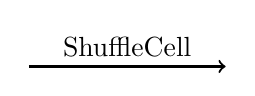
\begin{tikzpicture}[baseline=(current bounding box.center)]
            \draw[->, thick] (0,0) -- (2.5,0) node[midway, above] {ShuffleCell};
        \end{tikzpicture}
        \quad
        \begin{array}{|c|c|c|c|}
            \hline
            S_{0}  & S_{14} & S_{9}  & S_{7}  \\ \hline
            S_{10} & S_{4}  & S_{3}  & S_{13} \\ \hline
            S_{5}  & S_{11} & S_{12} & S_{2}  \\ \hline
            S_{15} & S_{1}  & S_{6}  & S_{8}  \\ \hline
        \end{array}
    \]
    \begin{center}
        Fig.3 : ShuffleCell.
    \end{center}

    The inverse of ShuffleCell (SC) is shown in Fig. 4.

    \[
        \renewcommand{\arraystretch}{1.5} % Adjust the row height
        \setlength{\tabcolsep}{0pt} % Remove extra padding between columns
        \begin{array}{|c|c|c|c|}
            \hline
            S_{0} & S_{4} & S_{8}  & S_{12} \\ \hline
            S_{1} & S_{5} & S_{9}  & S_{13} \\ \hline
            S_{2} & S_{6} & S_{10} & S_{14} \\ \hline
            S_{3} & S_{7} & S_{11} & S_{15} \\ \hline
        \end{array}
        \quad
        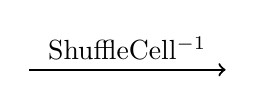
\begin{tikzpicture}[baseline=(current bounding box.center)]
            \draw[->, thick] (0,0) -- (2.5,0) node[midway, above] {ShuffleCell$^{-1}$};
        \end{tikzpicture}
        \quad
        \begin{array}{|c|c|c|c|}
            \hline
            S_{0}  & S_{5}  & S_{15} & S_{10} \\ \hline
            S_{7}  & S_{2}  & S_{8}  & S_{13} \\ \hline
            S_{14} & S_{11} & S_{1}  & S_{4}  \\ \hline
            S_{9}  & S_{12} & S_{6}  & S_{3}  \\ \hline
        \end{array}
    \]
    \begin{center}
        Fig.4 : ShuffleCell$^{-1}$
    \end{center}

    \subsubsection{MixColumn (\( \mathcal{MC} \))}
    The Cell vector in each column of State Matrix multiplies
    with a constant 4 × 4 binary matrix M, where M as given below:

    \begin{equation}
        \begin{bmatrix}
            0 & 1 & 1 & 1 \\
            1 & 0 & 1 & 1 \\
            1 & 1 & 0 & 1 \\
            1 & 1 & 1 & 0
        \end{bmatrix}
        \tag{1}
    \end{equation}

    \subsubsection{KeyAdd (\( \mathcal{S} \), \( \mathcal{RK$_{i}$} \)) }
    It is used bit-oriented. First, we should write round key as
    in (1) according to the rules. Second, the i-th m-bit round key
    RK$_{i}$ is XORed to m-bit of State Matrix S.


    \subsubsection{Key Schedule}
    The key schedule of Midori whose design is very simple.
    The whiten key WK in Midori are the initial key K, as in (3)
    \begin{equation}
        WK = K
        \tag{3}
    \end{equation}
    For the Midori64 algorithm, the initial key is divided into
    two 64-bit keys, that is K$_{0}$ and K$_{1}$ as K = K$_{0}$ || K$_{1}$. The sub-key
    of Midori64 for round i is K$_{i} = K$_{i mod 2} \oplus \( \mathcal{B$_{i}} \)

    \subsection{6 - Round integral distinguiser of midori}
    First, constructing a 4-round integral distinguisher in the
    direction of encryption with an active byte as shown in Fig. 5.

    % attack 6 round 
    \renewcommand{\arraystretch}{1.5} % Adjust the row height
\setlength{\tabcolsep}{0pt} % Remove extra padding between columns
\begin{center}
    \resizebox{\textwidth}{!}{%
        \(
        \begin{array}{|p{0.4cm}|p{0.4cm}|p{0.4cm}|p{0.4cm}|}
            \hline
            \( \mathcal{A} \) &  &  & \\ \hline
                              &  &  & \\ \hline
                              &  &  & \\ \hline
                              &  &  & \\ \hline
        \end{array}
        \hspace{2pt} % Decrease space here
        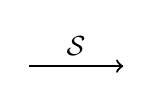
\begin{tikzpicture}[baseline={(current bounding box.center)}, scale=0.4]
            % Arrow from first grid to second grid
            \draw[->, thick] (0, 0) -- (3, 0)
            node[midway, above] {\( \mathcal{S} \)};
        \end{tikzpicture}
        \hspace{2pt} % Decrease space here
        \begin{array}{|p{0.4cm}|p{0.4cm}|p{0.4cm}|p{0.4cm}|}
            \hline
            \( \mathcal{A} \) &  &  & \\ \hline
                              &  &  & \\ \hline
                              &  &  & \\ \hline
                              &  &  & \\ \hline
        \end{array}
        \hspace{2pt} % Decrease space here
        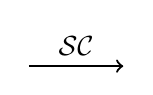
\begin{tikzpicture}[baseline={(current bounding box.center)}, scale=0.4]
            % Arrow from second grid to third grid
            \draw[->, thick] (0, 0) -- (3, 0)
            node[midway, above] {\( \mathcal{SC} \)};
        \end{tikzpicture}
        \hspace{2pt} % Decrease space here
        \begin{array}{|p{0.4cm}|p{0.4cm}|p{0.4cm}|p{0.4cm}|}
            \hline
            \( \mathcal{A} \) &  &  & \\ \hline
                              &  &  & \\ \hline
                              &  &  & \\ \hline
                              &  &  & \\ \hline
        \end{array}
        \hspace{2pt} % Decrease space here
        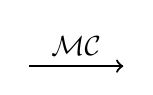
\begin{tikzpicture}[baseline={(current bounding box.center)}, scale=0.4]
            % Arrow from third grid to fourth grid
            \draw[->, thick] (0, 0) -- (3, 0)
            node[midway, above] {\( \mathcal{MC} \)};
        \end{tikzpicture}
        \hspace{2pt} % Decrease space here
        \begin{array}{|p{0.4cm}|p{0.4cm}|p{0.4cm}|p{0.4cm}|}
            \hline
                              &  &  & \\ \hline
            \( \mathcal{A} \) &  &  & \\ \hline
            \( \mathcal{A} \) &  &  & \\ \hline
            \( \mathcal{A} \) &  &  & \\ \hline
        \end{array}
        \)
        \hspace{2pt} % Decrease space here

        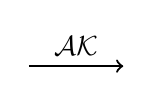
\begin{tikzpicture}[baseline={(current bounding box.center)}, scale=0.4]
            % Arrow from third grid to fourth grid
            \draw[->, thick] (0, 0) -- (3, 0)
            node[midway, above] {\( \mathcal{AK} \)};
        \end{tikzpicture}
        \hspace{2pt} % Decrease space here
        \begin{array}{|p{0.4cm}|p{0.4cm}|p{0.4cm}|p{0.4cm}|}
            \hline
                              &  &  & \\ \hline
            \( \mathcal{A} \) &  &  & \\ \hline
            \( \mathcal{A} \) &  &  & \\ \hline
            \( \mathcal{A} \) &  &  & \\ \hline
        \end{array}

    }
\end{center}
\vspace{15}
\resizebox{\textwidth}{!}{%
    \(
    % \begin{array}{|p{0.4cm}|p{0.4cm}|p{0.4cm}|p{0.4cm}|}
    % \hline
    % \( \mathcal{A} \) &  &  &  \\ \hline
    %  &  &  &  \\ \hline
    %  &  &  &  \\ \hline
    %  &  &  &  \\ \hline
    % \end{array}
    \hspace{2pt} % Decrease space here
    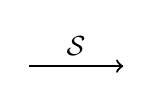
\begin{tikzpicture}[baseline={(current bounding box.center)}, scale=0.4]
        % Arrow from first grid to second grid
        \draw[->, thick] (0, 0) -- (3, 0)
        node[midway, above] {\( \mathcal{S} \)};
    \end{tikzpicture}
    \hspace{2pt} % Decrease space here
    \begin{array}{|p{0.4cm}|p{0.4cm}|p{0.4cm}|p{0.4cm}|}
        \hline
                          &  &  & \\ \hline
        \( \mathcal{A} \) &  &  & \\ \hline
        \( \mathcal{A} \) &  &  & \\ \hline
        \( \mathcal{A} \) &  &  & \\ \hline
    \end{array}
    \hspace{2pt} % Decrease space here
    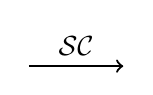
\begin{tikzpicture}[baseline={(current bounding box.center)}, scale=0.4]
        % Arrow from second grid to third grid
        \draw[->, thick] (0, 0) -- (3, 0)
        node[midway, above] {\( \mathcal{SC} \)};
    \end{tikzpicture}
    \hspace{2pt} % Decrease space here
    \begin{array}{|p{0.4cm}|p{0.4cm}|p{0.4cm}|p{0.4cm}|}
        \hline
         &                   &                   &                   \\ \hline
         &                   & \( \mathcal{A} \) &                   \\ \hline
         &                   &                   & \( \mathcal{A} \) \\ \hline
         & \( \mathcal{A} \) &                   &                   \\ \hline
    \end{array}
    \hspace{2pt} % Decrease space here
    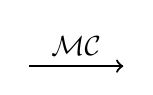
\begin{tikzpicture}[baseline={(current bounding box.center)}, scale=0.4]
        % Arrow from third grid to fourth grid
        \draw[->, thick] (0, 0) -- (3, 0)
        node[midway, above] {\( \mathcal{MC} \)};
    \end{tikzpicture}
    \hspace{2pt} % Decrease space here
    \begin{array}{|p{0.4cm}|p{0.4cm}|p{0.4cm}|p{0.4cm}|}
        \hline
         & \( \mathcal{A} \) & \( \mathcal{A} \) & \( \mathcal{A} \) \\ \hline
         & \( \mathcal{A} \) &                   & \( \mathcal{A} \) \\ \hline
         & \( \mathcal{A} \) & \( \mathcal{A} \) &                   \\ \hline
         &                   & \( \mathcal{A} \) & \( \mathcal{A} \) \\ \hline
    \end{array}
    \)
    \hspace{2pt} % Decrease space here

    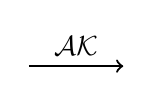
\begin{tikzpicture}[baseline={(current bounding box.center)}, scale=0.4]
        % Arrow from third grid to fourth grid
        \draw[->, thick] (0, 0) -- (3, 0)
        node[midway, above] {\( \mathcal{AK} \)};
    \end{tikzpicture}
    \hspace{2pt} % Decrease space here

    \begin{array}{|p{0.4cm}|p{0.4cm}|p{0.4cm}|p{0.4cm}|}
        \hline
         & \( \mathcal{A} \) & \( \mathcal{A} \) & \( \mathcal{A} \) \\ \hline
         & \( \mathcal{A} \) &                   & \( \mathcal{A} \) \\ \hline
         & \( \mathcal{A} \) & \( \mathcal{A} \) &                   \\ \hline
         &                   & \( \mathcal{A} \) & \( \mathcal{A} \) \\ \hline
    \end{array}
    \)

}
\end{center}
\vspace{15}
\resizebox{\textwidth}{!}{%
    \(
    % \begin{array}{|p{0.4cm}|p{0.4cm}|p{0.4cm}|p{0.4cm}|}
    % \hline
    % \( \mathcal{A} \) &  &  &  \\ \hline
    %  &  &  &  \\ \hline
    %  &  &  &  \\ \hline
    %  &  &  &  \\ \hline
    % \end{array}
    \hspace{2pt} % Decrease space here
    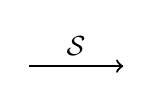
\begin{tikzpicture}[baseline={(current bounding box.center)}, scale=0.4]
        % Arrow from first grid to second grid
        \draw[->, thick] (0, 0) -- (3, 0)
        node[midway, above] {\( \mathcal{S} \)};
    \end{tikzpicture}
    \hspace{2pt} % Decrease space here
    \begin{array}{|p{0.4cm}|p{0.4cm}|p{0.4cm}|p{0.4cm}|}
        \hline
         & \( \mathcal{A} \) & \( \mathcal{A} \) & \( \mathcal{A} \) \\ \hline
         & \( \mathcal{A} \) &                   & \( \mathcal{A} \) \\ \hline
         & \( \mathcal{A} \) & \( \mathcal{A} \) &                   \\ \hline
         &                   & \( \mathcal{A} \) & \( \mathcal{A} \) \\ \hline
    \end{array}
    \)
    \hspace{2pt} % Decrease space here
    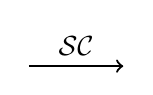
\begin{tikzpicture}[baseline={(current bounding box.center)}, scale=0.4]
        % Arrow from second grid to third grid
        \draw[->, thick] (0, 0) -- (3, 0)
        node[midway, above] {\( \mathcal{SC} \)};
    \end{tikzpicture}
    \hspace{2pt} % Decrease space here
    \begin{array}{|p{0.4cm}|p{0.4cm}|p{0.4cm}|p{0.4cm}|}
        \hline
                          &                   &                   &                   \\ \hline
        \( \mathcal{A} \) & \( \mathcal{A} \) &                   & \( \mathcal{A} \) \\ \hline
        \( \mathcal{A} \) & \( \mathcal{A} \) & \( \mathcal{A} \) &                   \\ \hline
        \( \mathcal{A} \) &                   & \( \mathcal{A} \) & \( \mathcal{A} \) \\ \hline
    \end{array}
    \hspace{2pt} % Decrease space here
    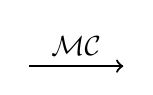
\begin{tikzpicture}[baseline={(current bounding box.center)}, scale=0.4]
        % Arrow from third grid to fourth grid
        \draw[->, thick] (0, 0) -- (3, 0)
        node[midway, above] {\( \mathcal{MC} \)};
    \end{tikzpicture}
    \hspace{2pt} % Decrease space here
    \begin{array}{|p{0.4cm}|p{0.4cm}|p{0.4cm}|p{0.4cm}|}
        \hline
        \( \mathcal{B} \) & \( \mathcal{B} \) & \( \mathcal{B} \) & \( \mathcal{B} \) \\ \hline
        \( \mathcal{B} \) & \( \mathcal{A} \) & \( \mathcal{B} \) & \( \mathcal{A} \) \\ \hline
        \( \mathcal{B} \) & \( \mathcal{A} \) & \( \mathcal{A} \) & \( \mathcal{B} \) \\ \hline
        \( \mathcal{B} \) & \( \mathcal{B} \) & \( \mathcal{A} \) & \( \mathcal{A} \) \\ \hline
    \end{array}
    \hspace{2pt} % Decrease space here

    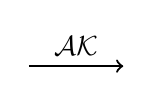
\begin{tikzpicture}[baseline={(current bounding box.center)}, scale=0.4]
        % Arrow from third grid to fourth grid
        \draw[->, thick] (0, 0) -- (3, 0)
        node[midway, above] {\( \mathcal{AK} \)};
    \end{tikzpicture}
    \hspace{2pt} % Decrease space here
    \begin{array}{|p{0.4cm}|p{0.4cm}|p{0.4cm}|p{0.4cm}|}
        \hline
        \( \mathcal{B} \) & \( \mathcal{B} \) & \( \mathcal{B} \) & \( \mathcal{B} \) \\ \hline
        \( \mathcal{B} \) & \( \mathcal{A} \) & \( \mathcal{B} \) & \( \mathcal{A} \) \\ \hline
        \( \mathcal{B} \) & \( \mathcal{A} \) & \( \mathcal{A} \) & \( \mathcal{B} \) \\ \hline
        \( \mathcal{B} \) & \( \mathcal{B} \) & \( \mathcal{A} \) & \( \mathcal{A} \) \\ \hline
    \end{array}

}
\end{center}
\vspace{15}
\resizebox{\textwidth}{!}{%
    \(
    % \begin{array}{|p{0.4cm}|p{0.4cm}|p{0.4cm}|p{0.4cm}|}
    % \hline
    % \( \mathcal{A} \) &  &  &  \\ \hline
    %  &  &  &  \\ \hline
    %  &  &  &  \\ \hline
    %  &  &  &  \\ \hline
    % \end{array}
    \hspace{2pt} % Decrease space here
    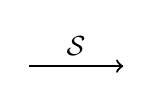
\begin{tikzpicture}[baseline={(current bounding box.center)}, scale=0.4]
        % Arrow from first grid to second grid
        \draw[->, thick] (0, 0) -- (3, 0)
        node[midway, above] {\( \mathcal{S} \)};
    \end{tikzpicture}
    \hspace{2pt} % Decrease space here
    \begin{array}{|p{0.4cm}|p{0.4cm}|p{0.4cm}|p{0.4cm}|}
        \hline
        \( \mathcal{U} \) & \( \mathcal{U} \) & \( \mathcal{U} \) & \( \mathcal{U} \) \\ \hline
        \( \mathcal{U} \) & \( \mathcal{A} \) & \( \mathcal{U} \) & \( \mathcal{A} \) \\ \hline
        \( \mathcal{U} \) & \( \mathcal{A} \) & \( \mathcal{A} \) & \( \mathcal{U} \) \\ \hline
        \( \mathcal{U} \) & \( \mathcal{U} \) & \( \mathcal{A} \) & \( \mathcal{A} \) \\ \hline
    \end{array}
    \hspace{2pt} % Decrease space here
    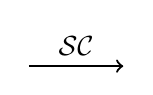
\begin{tikzpicture}[baseline={(current bounding box.center)}, scale=0.4]
        % Arrow from second grid to third grid
        \draw[->, thick] (0, 0) -- (3, 0)
        node[midway, above] {\( \mathcal{SC} \)};
    \end{tikzpicture}
    \hspace{2pt} % Decrease space here
    \begin{array}{|p{0.4cm}|p{0.4cm}|p{0.4cm}|p{0.4cm}|}
        \hline
        \( \mathcal{U} \) & \( \mathcal{U} \) & \( \mathcal{U} \) & \( \mathcal{U} \) \\ \hline
        \( \mathcal{A} \) & \( \mathcal{U} \) & \( \mathcal{U} \) & \( \mathcal{A} \) \\ \hline
        \( \mathcal{A} \) & \( \mathcal{A} \) & \( \mathcal{U} \) & \( \mathcal{U} \) \\ \hline
        \( \mathcal{A} \) & \( \mathcal{U} \) & \( \mathcal{A} \) & \( \mathcal{U} \) \\ \hline
    \end{array}
    \hspace{2pt} % Decrease space here
    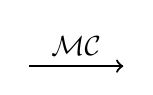
\begin{tikzpicture}[baseline={(current bounding box.center)}, scale=0.4]
        % Arrow from third grid to fourth grid
        \draw[->, thick] (0, 0) -- (3, 0)
        node[midway, above] {\( \mathcal{MC} \)};
    \end{tikzpicture}
    \hspace{2pt} % Decrease space here
    \begin{array}{|p{0.4cm}|p{0.4cm}|p{0.4cm}|p{0.4cm}|}
        \hline
        \( \mathcal{B} \) & \( \mathcal{U} \) & \( \mathcal{U} \) & \( \mathcal{U} \) \\ \hline
        \( \mathcal{U} \) & \( \mathcal{U} \) & \( \mathcal{U} \) & \( \mathcal{U} \) \\ \hline
        \( \mathcal{U} \) & \( \mathcal{U} \) & \( \mathcal{U} \) & \( \mathcal{U} \) \\ \hline
        \( \mathcal{U} \) & \( \mathcal{U} \) & \( \mathcal{U} \) & \( \mathcal{U} \) \\ \hline
    \end{array}
    \hspace{2pt} % Decrease space here

    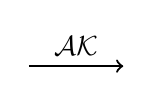
\begin{tikzpicture}[baseline={(current bounding box.center)}, scale=0.4]
        % Arrow from third grid to fourth grid
        \draw[->, thick] (0, 0) -- (3, 0)
        node[midway, above] {\( \mathcal{AK} \)};
    \end{tikzpicture}
    \hspace{2pt} % Decrease space here
    \begin{array}{|p{0.4cm}|p{0.4cm}|p{0.4cm}|p{0.4cm}|}
        \hline
        \( \mathcal{B} \) & \( \mathcal{U} \) & \( \mathcal{U} \) & \( \mathcal{U} \) \\ \hline
        \( \mathcal{U} \) & \( \mathcal{U} \) & \( \mathcal{U} \) & \( \mathcal{U} \) \\ \hline
        \( \mathcal{U} \) & \( \mathcal{U} \) & \( \mathcal{U} \) & \( \mathcal{U} \) \\ \hline
        \( \mathcal{U} \) & \( \mathcal{U} \) & \( \mathcal{U} \) & \( \mathcal{U} \) \\ \hline
    \end{array}

}
\end{center}


    \begin{center}
        Fig.5 : 4-Round integral distinguishers on Midori.
    \end{center}

    Second, constructing a 2-round integral distinguisher in
    the direction of decryption as shown in Fig. 6

    % attack 2 round
    \renewcommand{\arraystretch}{1.5} % Adjust the row height
\setlength{\tabcolsep}{0pt} % Remove extra padding between columns
\begin{center}
\resizebox{\textwidth}{!}{%
    \(
    \begin{array}{|p{0.4cm}|p{0.4cm}|p{0.4cm}|p{0.4cm}|}
    \hline
     &  &  &  \\ \hline
    \( \mathcal{\( A^* \)} \) &  & \( \mathcal{\( A^* \)} \) & \( \mathcal{\( A^* \)} \) \\ \hline
    \( \mathcal{\( A^* \)} \) & \( \mathcal{\( A^* \)} \) &  & \( \mathcal{\( A^* \)} \) \\ \hline
    \( \mathcal{\( A^* \)} \) & \( \mathcal{\( A^* \)} \) & \( \mathcal{\( A^* \)} \) &  \\ \hline
    \end{array}
    \hspace{2pt} % Decrease space here
    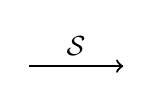
\begin{tikzpicture}[baseline={(current bounding box.center)}, scale=0.4]
        % Arrow from first grid to second grid
        \draw[->, thick] (0, 0) -- (3, 0)
            node[midway, above] {\( \mathcal{S} \)};
    \end{tikzpicture}
    \hspace{2pt} % Decrease space here
    \begin{array}{|p{0.4cm}|p{0.4cm}|p{0.4cm}|p{0.4cm}|}
    \hline
     &  &  &  \\ \hline
    \( \mathcal{\( A^* \)} \) &  & \( \mathcal{\( A^* \)} \) & \( \mathcal{\( A^* \)} \) \\ \hline
    \( \mathcal{\( A^* \)} \) & \( \mathcal{\( A^* \)} \) &  & \( \mathcal{\( A^* \)} \) \\ \hline
    \( \mathcal{\( A^* \)} \) & \( \mathcal{\( A^* \)} \) & \( \mathcal{\( A^* \)} \) &  \\ \hline
    \end{array}
    \hspace{2pt} % Decrease space here
    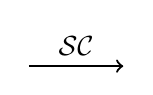
\begin{tikzpicture}[baseline={(current bounding box.center)}, scale=0.4]
        % Arrow from second grid to third grid
        \draw[->, thick] (0, 0) -- (3, 0)
            node[midway, above] {\( \mathcal{SC} \)};
    \end{tikzpicture}
    \hspace{2pt} % Decrease space here
    \begin{array}{|p{0.4cm}|p{0.4cm}|p{0.4cm}|p{0.4cm}|}
    \hline
     & \( \mathcal{\( A^* \)} \) & \( \mathcal{\( A^* \)} \) & \( \mathcal{\( A^* \)} \) \\ \hline
     &  & \( \mathcal{\( A^* \)} \) & \( \mathcal{\( A^* \)} \) \\ \hline
     & \( \mathcal{\( A^* \)} \) &  & \( \mathcal{\( A^* \)} \) \\ \hline
     & \( \mathcal{\( A^* \)} \) & \( \mathcal{\( A^* \)} \) &  \\ \hline
    \end{array}
    \hspace{2pt} % Decrease space here
    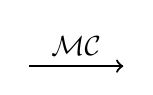
\begin{tikzpicture}[baseline={(current bounding box.center)}, scale=0.4]
        % Arrow from third grid to fourth grid
        \draw[->, thick] (0, 0) -- (3, 0)
            node[midway, above] {\( \mathcal{MC} \)};
    \end{tikzpicture}
    \hspace{2pt} % Decrease space here
    \begin{array}{|p{0.4cm}|p{0.4cm}|p{0.4cm}|p{0.5cm}|}
    \hline
     &  &  &  \\ \hline
     & \( \mathcal{A$_{2}$} \) &  &  \\ \hline
     &  & \( \mathcal{A$_{1}$} \) &  \\ \hline
     &  &  & \( \mathcal{A$_{3}$} \) \\ \hline
    \end{array}
    \hspace{2pt} % Decrease space here

    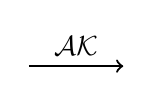
\begin{tikzpicture}[baseline={(current bounding box.center)}, scale=0.4]
        % Arrow from third grid to fourth grid
        \draw[->, thick] (0, 0) -- (3, 0)
            node[midway, above] {\( \mathcal{AK} \)};
    \end{tikzpicture}
    \hspace{2pt} % Decrease space here
    \begin{array}{|p{0.4cm}|p{0.4cm}|p{0.4cm}|p{0.5cm}|}
    \hline
     &  &  &  \\ \hline
     & \( \mathcal{A$_{2}$} \) &  &  \\ \hline
     &  &\( \mathcal{A$_{1}$} \) &  \\ \hline
     &  &  & \( \mathcal{A$_{3}$} \) \\ \hline
    \end{array}
    
}
\end{center}
\vspace{15}
\resizebox{\textwidth}{!}{%
    \(
    % \begin{array}{|p{0.4cm}|p{0.4cm}|p{0.4cm}|p{0.4cm}|}
    % \hline
    % \( \mathcal{A} \) &  &  &  \\ \hline
    %  &  &  &  \\ \hline
    %  &  &  &  \\ \hline
    %  &  &  &  \\ \hline
    % \end{array}
    \hspace{2pt} % Decrease space here
    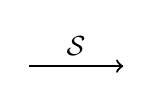
\begin{tikzpicture}[baseline={(current bounding box.center)}, scale=0.4]
        % Arrow from first grid to second grid
        \draw[->, thick] (0, 0) -- (3, 0)
            node[midway, above] {\( \mathcal{S} \)};
    \end{tikzpicture}
    \hspace{2pt} % Decrease space here
    \begin{array}{|p{0.4cm}|p{0.4cm}|p{0.4cm}|p{0.5cm}|}
    \hline
     &  &  &  \\ \hline
     & A$_{2}$ &  &  \\ \hline
     &  & A$_{1}$ &  \\ \hline
     &  &  & A$_{3}$ \\ \hline
    \end{array}
    \hspace{2pt} % Decrease space here
    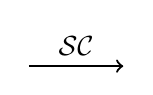
\begin{tikzpicture}[baseline={(current bounding box.center)}, scale=0.4]
        % Arrow from second grid to third grid
        \draw[->, thick] (0, 0) -- (3, 0)
            node[midway, above] {\( \mathcal{SC} \)};
    \end{tikzpicture}
    \hspace{2pt} % Decrease space here
    \begin{array}{|p{0.4cm}|p{0.4cm}|p{0.4cm}|p{0.4cm}|}
    \hline
     &  &  &  \\ \hline
    \( \mathcal{A$_{1}$} \) &  &  &  \\ \hline
    \( \mathcal{A$_{2}$} \) &  &  &  \\ \hline
    \( \mathcal{A$_{3}$} \) &  &  &  \\ \hline
    \end{array}
    \hspace{2pt} % Decrease space here
    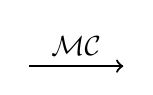
\begin{tikzpicture}[baseline={(current bounding box.center)}, scale=0.4]
        % Arrow from third grid to fourth grid
        \draw[->, thick] (0, 0) -- (3, 0)
            node[midway, above] {\( \mathcal{MC} \)};
    \end{tikzpicture}
    \hspace{2pt} % Decrease space here
    \begin{array}{|p{0.4cm}|p{0.4cm}|p{0.4cm}|p{0.4cm}|}
    \hline
     \( \mathcal{A} \) &  &  &  \\ \hline
     &  &  &  \\ \hline
     &  &  &  \\ \hline
     &  &  & \\ \hline
    \end{array}
    \)
    \hspace{2pt} % Decrease space here

    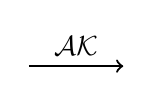
\begin{tikzpicture}[baseline={(current bounding box.center)}, scale=0.4]
        % Arrow from third grid to fourth grid
        \draw[->, thick] (0, 0) -- (3, 0)
            node[midway, above] {\( \mathcal{AK} \)};
    \end{tikzpicture}
    \hspace{2pt} % Decrease space here
   
    \begin{array}{|p{0.4cm}|p{0.4cm}|p{0.4cm}|p{0.4cm}|}
    \hline
     \( \mathcal{A} \) &  &  &  \\ \hline
     & &  &  \\ \hline
     &  &   &  \\ \hline
     &  &  &  \\ \hline
    \end{array}
    \)
    
}

\hspace{2pt} % Decrease space here

\[
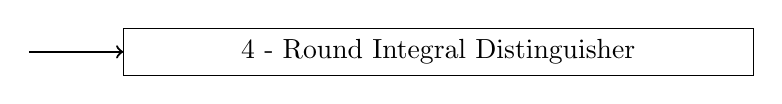
\begin{tikzpicture}[baseline={(current bounding box.center)}, scale=0.4]
    % Arrow from left to the box
    \draw[->, thick] (0, 0) -- (3, 0)
        node[midway, above] {};
    % Add the box at the end of the arrow
    \draw (3, -0.75) rectangle ++(20, 1.5) node[pos=.5] {4 - Round Integral Distinguisher};
\end{tikzpicture}
\]

\end{center}

    \begin{center}
        Fig.6 : 6-Round integral distinguishers on Midori.
    \end{center}

    Lemma 1: Taking nine 4 bits  cells in plaintext state S$_1{^0}$ ,
    S$_2{^0}$ ,
    S$_3{^0}$ ,
    S$_6{^0}$ ,
    S$_7{^0}$ ,
    S$_9{^0}$ ,
    S$_{11}{^0}$ ,
    S$_{13}{^0}$ ,
    S$_{14}{^0}$ as active A that
    traverse all values, and other 4 bits cells are constants C. After two
    rounds of encryption, we get $2^{32}$ sets and in each set the byte
    of S$_0{^2}$ will traverse all values, and the other bytes are
    constants C.

    Proof. It's just a case of proving when S$_1}$, S$_2}$, S$_3}$ take all
    values in equation given below. After $2^{12}$ vectors $(0, S$_1}$, S$_2}$, S$_3}$)^T$ are
    transformed by MixColumn(MC), $2^{8}$ sets are obtained and
    the first component of each set takes all values of 0 to 15 and
    others are constants C.


    \[
        \begin{bmatrix}
            0 & 1 & 1 & 1 \\
            1 & 0 & 1 & 1 \\
            1 & 1 & 0 & 1 \\
            1 & 1 & 1 & 0 \\
        \end{bmatrix}
        \begin{bmatrix}
            0     \\
            S$_1$ \\
            S$_2$ \\
            S$_3$ \\
        \end{bmatrix}
        =
        \begin{bmatrix}
            S$_1$ \oplus S$_2$ \oplus S$_3$ \\
            S$_2$ \oplus S$_3$              \\
            S$_1$  \oplus S$_3$             \\
            S$_1$ \oplus S$_2$              \\
        \end{bmatrix}
    \]


    Let $S_1$ \oplus $S_2$ \oplus $S_3$ = $t_1$, S$_2$ \oplus S$_3$ = $t_2$, S$_1$ \oplus S$_3$ = $t_3$ which vectors
    are pairwise independence. The fourth vector is S$_1$ \oplus S$_2$ = t$_1$ \oplus t$_2$  that is the linear combination of the second
    component and the third component. Therefore, when S$_2$ ,S$_3$ are  constants  the first vector in the set takes all values of
    0 to 15. This collection has a total of $2^8$.
    This property is applied to the first round and second
    round of transformation, so we get the Lemma 1

    \newpage
    \section{S-box Analysis of Midori64}
    
\noindent The Midori64 cipher is a lightweight block cipher designed for
energy-efficient applications. It employs a 4-bit S-box in its substitution
layer, which plays a critical role in ensuring the cipher's security. The S-box
used in Midori64, along with its Differential Distribution Table (DDT), is
analyzed to evaluate its resistance to differential cryptanalysis.

\subsection*{Midori64 S-box}
\noindent The S-box used in the Midori64 cipher is shown below:

\begin{table}[h!]
	\centering
	\setlength{\tabcolsep}{8pt}
	\renewcommand{\arraystretch}{1.5}
	\begin{tabular}{|c|c|c|c|c|c|c|c|c|c|c|c|c|c|c|c|c|}
\hline
x & 0 & 1 & 2 & 3 & 4 & 5 & 6 & 7 & 8 & 9 & A & B & C & D & E & F \\
\hline
S(x) & C & A & D & 3 & E & B & F & 7 & 8 & 9 & 1 & 5 & 0 & 2 & 4 & 6 \\
\hline
\end{tabular} % Generated from Python
	\hspace{2pt}
	\caption{Midori64 S-box}
\end{table}

\subsection{Differential Distribution Table (DDT)}
\noindent The Differential Distribution Table (DDT) of the S-box is presented
below. It quantifies the probability of each output difference occurring for a
given input difference.

\begin{table}[h!]
	\centering
	\label{tab:ddt}
	\caption{Differential Distribution Table (DDT)}
	\setlength{\tabcolsep}{8pt}
	\hspace{2pt}
	\begin{tabular}{c|cccccccccccccccc}
in /\ out & 0 & 1 & 2 & 3 & 4 & 5 & 6 & 7 & 8 & 9 & A & B & C & D & E & F \\
\hline
0 & 16 & - & - & - & - & - & - & - & - & - & - & - & - & - & - & - \\
1 & - & 2 & 4 & - & 2 & 2 & 2 & - & 2 & - & - & - & - & - & 2 & - \\
2 & - & 4 & - & - & 4 & - & - & - & - & 4 & - & - & 4 & - & - & - \\
3 & - & - & - & - & 2 & - & 4 & 2 & 2 & 2 & - & - & - & 2 & - & 2 \\
4 & - & 2 & 4 & 2 & 2 & 2 & - & - & 2 & - & - & 2 & - & - & - & - \\
5 & - & 2 & - & - & 2 & - & - & 4 & - & 2 & 4 & - & 2 & - & - & - \\
6 & - & 2 & - & 4 & - & - & - & 2 & 2 & - & - & - & 2 & 2 & - & 2 \\
7 & - & - & - & 2 & - & 4 & 2 & - & - & - & - & 2 & - & 4 & 2 & - \\
8 & - & 2 & - & 2 & 2 & - & 2 & - & - & 2 & - & 2 & 2 & - & 2 & - \\
9 & - & - & 4 & 2 & - & 2 & - & - & 2 & 2 & - & 2 & 2 & - & - & - \\
A & - & - & - & - & - & 4 & - & - & - & - & 4 & - & - & 4 & - & 4 \\
B & - & - & - & - & 2 & - & - & 2 & 2 & 2 & - & 4 & - & 2 & - & 2 \\
C & - & - & 4 & - & - & 2 & 2 & - & 2 & 2 & - & - & 2 & - & 2 & - \\
D & - & - & - & 2 & - & - & 2 & 4 & - & - & 4 & 2 & - & - & 2 & - \\
E & - & 2 & - & - & - & - & - & 2 & 2 & - & - & - & 2 & 2 & 4 & 2 \\
F & - & - & - & 2 & - & - & 2 & - & - & - & 4 & 2 & - & - & 2 & 4 \\
\end{tabular} % Generated from Python
\end{table}

\newpage
\textbf{Value Counts in the DDT:}

The distribution of values in the Difference Distribution Table (DDT) is as follows:
\begin{table}[h!]
	\centering
	\setlength{\tabcolsep}{5pt}
	\begin{tabular}{|c|c|}
		\hline
		\textbf{Value} & \textbf{Count} \\ \hline
		0              & 159            \\ \hline
		2              & 72             \\ \hline
		4              & 24             \\ \hline
		16             & 1              \\ \hline
	\end{tabular}
\end{table}

\subsection{Differential Distribution Table (DDT) Analysis}

\subsubsection*{1. Differential Uniformity}
\begin{itemize}
	\item \textbf{Observation:} The maximum value in the DDT is 4, which is the
	      largest count (excluding the first row). This means that the
	      \textit{differential uniformity} is \( \Delta_{\text{max}} = 4 \).

	\item \textbf{Conclusion:} The differential uniformity of 4 indicates that
	      the cipher is somewhat resistant to differential cryptanalysis, but it is
	      not as strong as S-boxes with \( \Delta_{\text{max}} = 4 \) (e.g., AES)
	      which occurs only once in row.  As in Midori cipher's DDT contains  \(
	      \Delta_{\text{max}} = 4 \) more than one for the row.  However, for
	      lightweight ciphers like Midori, this trade-off is acceptable, as it
	      balances security with efficiency.
\end{itemize}

\subsubsection*{2. Uniform Distribution of Values}
\begin{itemize}
	\item
	      \textbf{Observation:} The values in the DDT are relatively evenly distributed,
	      and there are no particular input-output differential pairs that dominate the
	      table.
	\item
	      \textbf{Conclusion:} This suggests that the S-box does not have significant
	      biases or vulnerabilities that would make it easier for attackers to exploit
	      specific differentials. This balanced distribution enhances the cipher's
	      resistance to differential cryptanalysis.
\end{itemize}

\subsubsection*{3. Null Entries in the DDT}
\begin{itemize}
	\item
	      \textbf{Observation:} Several entries in the DDT are 0, which means
	      that certain input differences do not produce specific output
	      differences. This occurs in rows like the first and others.
	\item
	      \textbf{Conclusion:} Null entries limit an attacker’s ability to craft
	      specific differential trails, as they indicate that some differentials
	      cannot happen. This property adds an extra layer of security to the
	      S-box.
\end{itemize}

\subsubsection*{4. Symmetry}
\begin{itemize}
	\item
	      \textbf{Observation:} The DDT is symmetric, i.e., if \( D(x, y) \) is an entry,
	      then \( D(y, x) \) is also an entry.
	\item
	      \textbf{Conclusion:} This symmetry is expected for well-designed S-boxes and
	      confirms the correctness of the DDT, ensuring that the cryptographic function
	      behaves consistently in both directions (input to output and vice versa).
\end{itemize}

\subsubsection*{5. Compliance with DDT Properties}
The following propositions hold true for the DDT of Midori64:
\begin{itemize}
	\item \textbf{Proposition 1:} Every entry in the DDT is a non-negative even
	      integer between 0 and \( 2^n \).
	\item \textbf{Proposition 2:} The top-left entry of the DDT is \( 2^n \).
	\item \textbf{Proposition 3:} The first row consists of all zeros except the
	      first entry, which is \( 2^n \).
	\item \textbf{Proposition 4:} The first column consists of all zeros except
	      the first entry, which is \( 2^n \).
	\item \textbf{Proposition 5:} The sum of the entries of each row is \( 2^n \).
	\item \textbf{Proposition 6:} If the S-box is bijective, then every row and
	      column of the DDT adds up to \( 2^n \).
\end{itemize}

The DDT of the Midori64 S-box adheres to these properties, which confirms that
the S-box is well-structured and complies with the expected cryptographic
behaviors.

\subsubsection*{Comparative Analysis with Other Ciphers}
\begin{table}[h!]
	\centering
	\renewcommand{\arraystretch}{1.5} % Adjust row height
	\setlength{\tabcolsep}{5pt} % Adjust column spacing
	\caption{Comparison of DDT Properties Across Ciphers}
	\label{tab:ddt_comparison}
	\resizebox{\textwidth}{!}{%
		\begin{tabular}{|c|c|c|c|c|c|c|}
			\hline
			\textbf{Cipher Name} & \textbf{Number of 0's} & \textbf{Number of 2's} & \textbf{Number of 4's} & \textbf{Number of 16's} & \textbf{Differential Uniformity} \\ \hline
			Pyjamask-128         & -                      & -                      & -                      & -                       & -                                \\ \hline
			Square               & 159                    & 72                     & 24                     & 1                       & 4                                \\ \hline
			PRESENT              & -                      & -                      & -                      & -                       & -                                \\ \hline
			PRINCE               & -                      & -                      & -                      & -                       & -                                \\ \hline
			KLEIN                & -                      & -                      & -                      & -                       & -                                \\ \hline
			LED                  & -                      & -                      & -                      & -                       & -                                \\ \hline
			BACKSHEESH           & 198                    & 0                      & 56                     & 2                       & 4                                \\ \hline
			Midori               & 159                    & 72                     & 24                     & 1                       & 4                                \\ \hline
			GIFT                 & -                      & -                      & -                      & -                       & -                                \\ \hline
			PRINTcipher          & -                      & -                      & -                      & -                       & -                                \\ \hline
			Rectangle            & -                      & -                      & -                      & -                       & -                                \\ \hline
		\end{tabular}%
	}
\end{table}



\subsubsection*{Conclusion}

The Midori64 S-box offers a reasonable trade-off between security and
efficiency, making it suitable for lightweight cryptographic applications. While
it does not have the optimal differential uniformity of \( \Delta_{\text{max}} = 2 \)
seen in AES, it remains secure against differential cryptanalysis and other
attacks due to its balanced distribution and structural properties.

\subsection{Linear Approximation Table (LAT) Analysis of the Midori64 S-box}

\noindent The Linear Approximation Table (LAT) for the S-box is a key component
for analyzing the resistance of the S-box to linear cryptanalysis. It quantifies
how well the S-box behaves under linear approximations, with lower values
indicating better resistance. The LAT for the Midori64 S-box is shown below:

\begin{table}[h!]
	\centering
	\label{tab:lat}
	\caption{Linear Approximation Table (LAT) for the Midori64 S-box}
	\setlength{\tabcolsep}{8pt}
	\vspace{12pt}
	    \begin{tabular}{|c|cccccccccccccccc|}
        \hline
          & 0 & 1 & 2 & 3 & 4 & 5 & 6 & 7 & 8 & 9 & a & b & c & d & e & f \\
        \hline
        0 & 8 & . & . & . & . & . & . & . & . & . & . & . & . & . & . & . \\
        1 & . & 2 & 4 & 2 & -2 & . & 2 & . & -2 & . & 2 & . & 4 & -2 & . & -2 \\
        2 & . & 4 & . & . & 4 & . & . & . & -4 & . & . & . & . & 4 & . & . \\
        3 & . & 2 & . & 2 & -2 & . & 2 & 4 & 2 & -4 & -2 & . & . & 2 & . & 2 \\
        4 & . & -2 & 4 & -2 & 2 & . & -2 & . & -2 & -4 & -2 & . & . & -2 & . & 2 \\
        5 & . & . & . & . & . & . & . & . & . & . & -4 & -4 & . & . & 4 & -4 \\
        6 & . & 2 & . & 2 & -2 & . & 2 & -4 & -2 & . & -2 & . & -4 & -2 & . & 2 \\
        7 & . & . & . & 4 & . & . & -4 & . & . & . & . & -4 & . & . & -4 & . \\
        8 & . & -2 & -4 & 2 & -2 & . & -2 & . & -4 & -2 & . & 2 & 2 & . & 2 & . \\
        9 & . & . & . & -4 & -4 & . & . & . & -2 & 2 & -2 & -2 & 2 & 2 & -2 & 2 \\
        a & . & 2 & . & -2 & -2 & -4 & -2 & . & . & -2 & 4 & -2 & -2 & . & 2 & . \\
        b & . & . & . & . & . & -4 & . & -4 & 2 & -2 & -2 & 2 & 2 & 2 & -2 & -2 \\
        c & . & 4 & . & . & . & . & -4 & . & 2 & 2 & -2 & 2 & 2 & -2 & 2 & 2 \\
        d & . & -2 & 4 & 2 & -2 & . & -2 & . & . & 2 & . & 2 & -2 & 4 & 2 & . \\
        e & . & . & . & . & . & 4 & . & -4 & 2 & -2 & 2 & -2 & 2 & 2 & 2 & 2 \\
        f & . & -2 & . & 2 & 2 & -4 & 2 & . & . & 2 & . & -2 & 2 & . & 2 & 4 \\
        \hline
    \end{tabular}
\end{table}

\textbf{Value Counts in the Linear Approximation Table (LAT)}
This table represents the counts of each value observed in the Linear
Approximation Table (LAT) for the Midori64 S-box.

\begin{table}[h!]
	\centering
	\setlength{\tabcolsep}{5pt}
	\begin{tabular}{|c|c|}
		\hline
		\textbf{Value} & \textbf{Count} \\
		\hline
		-4             & 21             \\
		-2             & 44             \\
		0              & 123            \\
		2              & 52             \\
		4              & 15             \\
		8              & 1              \\
		\hline
	\end{tabular}
\end{table}

\subsection*{LAT Analysis}

\subsubsection*{1. Linear Bias and Distribution of Values}
\begin{itemize}
	\item \textbf{Observation:} The values in the LAT table are spread between
	      positive and negative numbers. A few entries show larger values such as $\pm
		      4$ and $\pm 2$, which represent the linear bias of the approximation. Most
	      values are closer to 0, indicating weaker linear approximations.
	\item \textbf{Conclusion:} The distribution of values suggests that the
	      S-box of Midori64 is somewhat resistant to linear cryptanalysis. Ideally,
	      the values should be close to 0 for most of the entries, which is the case
	      here, though some larger biases may still indicate potential
	      vulnerabilities.
\end{itemize}

\subsubsection*{2. Symmetry in LAT}
\begin{itemize}
	\item \textbf{Observation:} The LAT is symmetric, i.e., the value at
	      position $(i, j)$ is equal to the value at position $(j, i)$, which is
	      expected from a well-designed S-box.
	\item \textbf{Conclusion:} The symmetry of the LAT confirms that the
	      Midori64 S-box behaves consistently in both directions (input to output and
	      vice versa), which is a desirable property for cryptographic functions and
	      indicates correctness in design.
\end{itemize}

\subsubsection*{3. Even Integer Entries in LAT}
\begin{itemize}
	\item \textbf{Observation:} All the entries in the LAT are even integers, as
	      expected from a bijective S-box. This property holds true for the Midori64
	      S-box, which confirms that the S-box is a bijection.
	\item \textbf{Conclusion:} The fact that all LAT entries are even integers,
	      and the first row and column (except the upper-left entry) consist of zeros,
	      is a strong indicator that the S-box is bijective. This makes the S-box more
	      secure against linear cryptanalysis.
\end{itemize}

\subsubsection*{4. Compliance with LAT Properties}
\begin{itemize}
	\item \textbf{Observation:} The first row and the first column are zeros,
	      except for the upper-left entry, which is $2^{n-1}$, indicating that the
	      S-box follows the LAT properties of bijective S-boxes.
	\item \textbf{Conclusion:} The Midori64 S-box adheres to the properties
	      expected from a bijective S-box. This is a positive feature, enhancing its
	      cryptographic strength by ensuring that no biases are introduced through
	      linear approximations.
\end{itemize}


\subsection*{Comparison with Other Ciphers}

\begin{table}[h!]
	\centering
	\renewcommand{\arraystretch}{1.5} % Adjust row height
	\setlength{\tabcolsep}{5pt} % Adjust column spacing
	\caption{Comparison of LAT Properties Across Ciphers}
	\label{tab:ddt_comparison}
	\resizebox{\textwidth}{!}{%
		\begin{tabular}{|c|c|c|c|c|c|c|}
			\hline
			\textbf{Cipher Name} & \textbf{Number of -4's} & \textbf{Number of -2's} & \textbf{Number of 0's} & \textbf{Number of 2's} & \textbf{Number of 4's} & \textbf{Number of 8's} \\ \hline
			Pyjamask-128         & 18                      & 52                      & 122                    & 44                     & 19                     & 1                      \\ \hline
			Square               & -                       & -                       & -                      & -                      & -                      & -                      \\ \hline
			PRESENT              & -                       & -                       & -                      & -                      & -                      & -                      \\ \hline
			PRINCE               & -                       & -                       & -                      & -                      & -                      & -                      \\ \hline
			KLEIN                & -                       & -                       & -                      & -                      & -                      & -                      \\ \hline
			LED                  & -                       & -                       & -                      & -                      & -                      & -                      \\ \hline
			BACKSHEESH           & 30                      & 0                       & 198                    & 0                      & 26                     & 2                      \\ \hline
			Midori               & -21                     & 44                      & 123                    & 52                     & 15                     & 1                      \\ \hline
			PUFFIN               & -                       & -                       & -                      & -                      & -                      & -                      \\ \hline
			GIFT                 & -                       & -                       & -                      & -                      & -                      & -                      \\ \hline
			PRINTcipher          & -                       & -                       & -                      & -                      & -                      & -                      \\ \hline
			Rectangle            & -                       & -                       & -                      & -                      & -                      & -                      \\ \hline
		\end{tabular}%
	}
\end{table}

\subsection*{Conclusion}

\noindent The Midori64 S-box strikes a balance between security and efficiency,
making it suitable for lightweight cryptographic applications. Although its LAT
does show some biases, the values are relatively small, and the overall
resistance to linear cryptanalysis is reasonable. The bijective nature of the
S-box, along with its symmetry and even integer entries, further contributes to
its security. While the Midori64 S-box may not be as optimal as the AES S-box in
terms of linear approximation resistance, it offers a good trade-off between
security and computational efficiency, which is crucial for lightweight
cryptography.


    \section*{Acknowledgment}
    In this term paper, we have not implemented the MILP (Mixed Integer Linear
    Programming) model for differential trail generation. Instead, we have
    referred directly to the results presented in the paper titled "MILP-Based
    Differential Cryptanalysis on Round-Reduced Midori64" by Jiageng Cheng,
    Xinyu Sun, and Meiqin Wang. For further details on the MILP trails, please
    see the original paper available at MILP-Based Differential Cryptanalysis on
    Round-Reduced Midori64. \cite{zhao2020}


    \newpage
    \section{Differential Attack on 11-Round Midori64}

    \subsection{The Property of Probability for Round Function}

    \textbf{Property 1:} Consider four cells of the intermediate state of SC with any input difference and any output difference. However, we want one cell of these four with zero difference after the MC operation. For example, let $X\{3, 6, 9, 12\}$ denote the positions (3, 6, 9, 12) before the SC operation, and $Y\{3, 6, 9, 12\}$, $Z\{8, 9, 10, 11\}$, $W\{8, 9, 10, 11\}$ denote the corresponding positions after SC, SFC, and MC operations, respectively. Let $\Delta w_{11} = 0$, then $\Delta z_8 = \Delta z_9 \oplus \Delta z_{10}$ with the probability of $\frac{1}{16} = 2^{-4}$. Let $P((?, ?, ?, ?) \to (?, ?, ?, 0))$ denote $P(\text{SC}(?, ?, ?, ?) \to \text{MC}(?, ?, ?, ?) = (?, ?, ?, 0))$. So, $P((?, ?, ?, ?) \to (?, ?, ?, 0)) = 2^{-4}$. Since $? \in \{0, 1, \dots, 15\}$ and $\ast \in \{1, 2, \dots, 15\}$, we can obtain $P((?, ?, ?, ?) \to (?, ?, \ast, 0)) = \frac{15}{16} \cdot \frac{1}{16} \approx 2^{-4.09}$. Similarly, $P((?, ?, ?, ?) \to (?, \ast, \ast, 0)) \approx 2^{-4.19}$, and $P((?, ?, ?, ?) \to (\ast, \ast, \ast, 0)) \approx 2^{-4.28}$.

    \textbf{Property 2:} Consider four cells of the intermediate state of SC with any input difference and any output difference. However, we want no less than one cell of these four with non-zero difference after the MC operation. We can obtain $P((?, ?, ?, ?) \to (?, ?, ?, \ast)) = \frac{15}{16} \approx 2^{-0.09}$. Similarly, $P((?, ?, ?, ?) \to (?, ?, \ast, \ast)) \approx 2^{-0.19}$, and $P((?, ?, ?, ?) \to (?, \ast, \ast, \ast)) \approx 2^{-0.28}$.

    \textbf{Property 3:} Consider four cells of SC with two arbitrary input differences and two non-zero differences; then, we want to get two zero differences after the MC operation. We can obtain $P((?, ?, \ast, \ast) \to (\ast, \ast, 0, 0)) = \frac{1}{16} \cdot \frac{1}{16} = 2^{-8}$ and $P((?, ?, \ast, \ast) \to (?, ?, 0, 0)) \approx 2^{-7.81}$.

    \textbf{Property 4:} If there are three cells with any or any non-zero input differences of SC and the same non-zero output differences of SC, we can obtain $P((?, ?, ?, 0) \to (11, 0, 0, 0)) = \frac{15}{16} \cdot \frac{1}{16} \cdot \frac{1}{16} \approx 2^{-8.09}$ and $P((\ast, \ast, \ast, 0) \to (12, 0, 0, 0)) \approx 2^{-7.81}$.

    \begin{table}[h!]
        \centering
        \caption{5-round differential path of Midori64 with probabilities $2^{-52}$ and $2^{-58}$.}
        \begin{tabular}{@{}clclc@{}}
            \toprule
            \textbf{Input Round} & \textbf{Input Differential-1}    & \textbf{Probability} & \textbf{Input Differential-2} & \textbf{Probability} \\ \midrule
            1                    & $\alpha$000 0000 00$\beta$0 0000 & 1                    & $\delta$000 0000 0000 0000    & 1                    \\
            2                    & 2200 0000 0000 0000              & $2^{-4}$             & 0AAA 0000 0000 0000           & $2^{-2}$             \\
            3                    & 0440 1110 0000 0000              & $2^{-8}$             & 0000 5550 A0AA AA0A           & $2^{-8}$             \\
            4                    & 2202 0202 0202 2202              & $2^{-20}$            & 05AF 0AA0 AA7D 0A0A           & $2^{-26}$            \\
            5                    & 0400 0011 0001 1100              & $2^{-40}$            & 5000 0077 00A0 5000           & $2^{-48}$            \\
            6                    & 0000 0022 0032 2200              & $2^{-52}$            & AA00 0000 FF5A 0555           & $2^{-58}$            \\ \bottomrule
        \end{tabular}
        \vspace{0.3cm}
        \begin{flushleft}
            $\alpha, \beta \in \{1,4,9,C\}$ and $\delta \in \{5,A,D,F\}.$
        \end{flushleft}
    \end{table}
    \newpage
    %  fig 1 differential attack
    \text{FIGURE 1. A 5-round differential path with probability of $2^{-58}$}

\renewcommand{\arraystretch}{1.5} % Adjust the row height
\setlength{\tabcolsep}{0pt} % Remove extra padding between columns

\begin{center}
    \resizebox{\textwidth}{!}{%
        \(
        \begin{array}{|p{0.5cm}|p{0.5cm}|p{0.5cm}|p{0.5cm}|}
            \hline
            \delta &  &  & \\ \hline
                   &  &  & \\ \hline
                   &  &  & \\ \hline
                   &  &  & \\ \hline
        \end{array}
        \hspace{2pt} % Decrease space here
        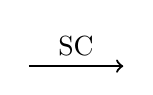
\begin{tikzpicture}[baseline={(current bounding box.center)}, scale=0.4]
            % Arrow from first grid to second grid
            \draw[->, thick] (0, 0) -- (3, 0)
            node[midway, above] {SC};
        \end{tikzpicture}
        \hspace{2pt} % Decrease space here
        \begin{array}{|p{0.5cm}|p{0.5cm}|p{0.5cm}|p{0.5cm}|}
            \hline
            A &  &  & \\ \hline
              &  &  & \\ \hline
              &  &  & \\ \hline
              &  &  & \\ \hline
        \end{array}
        \hspace{2pt} % Decrease space here
        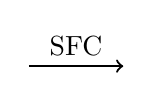
\begin{tikzpicture}[baseline={(current bounding box.center)}, scale=0.4]
            % Arrow from second grid to third grid
            \draw[->, thick] (0, 0) -- (3, 0)
            node[midway, above] {SFC};
        \end{tikzpicture}
        \hspace{2pt} % Decrease space here
        \begin{array}{|p{0.5cm}|p{0.5cm}|p{0.5cm}|p{0.5cm}|}
            \hline
            A &  &  & \\ \hline
              &  &  & \\ \hline
              &  &  & \\ \hline
              &  &  & \\ \hline
        \end{array}
        \hspace{2pt} % Decrease space here
        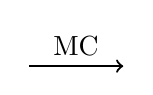
\begin{tikzpicture}[baseline={(current bounding box.center)}, scale=0.4]
            % Arrow from third grid to fourth grid
            \draw[->, thick] (0, 0) -- (3, 0)
            node[midway, above] {MC};
        \end{tikzpicture}
        \hspace{2pt} % Decrease space here
        \begin{array}{|p{0.5cm}|p{0.5cm}|p{0.5cm}|p{0.5cm}|}
            \hline
              &  &  & \\ \hline
            A &  &  & \\ \hline
            A &  &  & \\ \hline
            A &  &  & \\ \hline
        \end{array}
        \)
        \hspace{2pt} % Decrease space here

        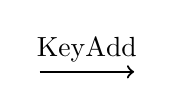
\begin{tikzpicture}[baseline={(current bounding box.center)}, scale=0.4]
            % Arrow from third grid to fourth grid
            \draw[->, thick] (0, 0) -- (3, 0)
            node[midway, above] {KeyAdd};
        \end{tikzpicture}

    }
\end{center}
\begin{center}
    \resizebox{\textwidth}{!}{%
        \(
        \begin{array}{|p{0.5cm}|p{0.5cm}|p{0.5cm}|p{0.5cm}|}
            \hline
              &  &  & \\ \hline
            A &  &  & \\ \hline
            A &  &  & \\ \hline
            A &  &  & \\ \hline
        \end{array}
        \hspace{2pt} % Decrease space here
        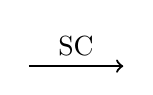
\begin{tikzpicture}[baseline={(current bounding box.center)}, scale=0.4]
            % Arrow from first grid to second grid
            \draw[->, thick] (0, 0) -- (3, 0)
            node[midway, above] {SC};
        \end{tikzpicture}
        \hspace{2pt} % Decrease space here
        \begin{array}{|p{0.5cm}|p{0.5cm}|p{0.5cm}|p{0.5cm}|}
            \hline
              &  &  & \\ \hline
            5 &  &  & \\ \hline
            A &  &  & \\ \hline
            A &  &  & \\ \hline
        \end{array}
        \hspace{2pt} % Decrease space here
        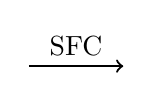
\begin{tikzpicture}[baseline={(current bounding box.center)}, scale=0.4]
            % Arrow from second grid to third grid
            \draw[->, thick] (0, 0) -- (3, 0)
            node[midway, above] {SFC};
        \end{tikzpicture}
        \hspace{2pt} % Decrease space here
        \begin{array}{|p{0.5cm}|p{0.5cm}|p{0.5cm}|p{0.5cm}|}
            \hline
             &   &   &   \\ \hline
             &   & A &   \\ \hline
             &   &   & A \\ \hline
             & 5 &   &   \\ \hline
        \end{array}
        \hspace{2pt} % Decrease space here
        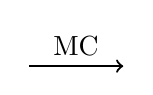
\begin{tikzpicture}[baseline={(current bounding box.center)}, scale=0.4]
            % Arrow from third grid to fourth grid
            \draw[->, thick] (0, 0) -- (3, 0)
            node[midway, above] {MC};
        \end{tikzpicture}
        \hspace{2pt} % Decrease space here
        \begin{array}{|p{0.5cm}|p{0.5cm}|p{0.5cm}|p{0.5cm}|}
            \hline
             & 5 & A & A \\ \hline
             & 5 &   & A \\ \hline
             & 5 & A &   \\ \hline
             &   & A & A \\ \hline
        \end{array}
        \)
        \hspace{2pt} % Decrease space here
        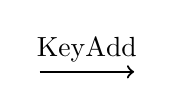
\begin{tikzpicture}[baseline={(current bounding box.center)}, scale=0.4]
            % Arrow from third grid to fourth grid
            \draw[->, thick] (0, 0) -- (3, 0)
            node[midway, above] {KeyAdd};
        \end{tikzpicture}

    }
\end{center}
\begin{center}
    \resizebox{\textwidth}{!}{%
        \(
        \begin{array}{|p{0.5cm}|p{0.5cm}|p{0.5cm}|p{0.5cm}|}
            \hline
             & 5 & A & A \\ \hline
             & 5 &   & A \\ \hline
             & 5 & A &   \\ \hline
             &   & A & A \\ \hline
        \end{array}
        \hspace{2pt} % Decrease space here
        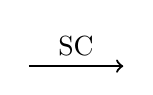
\begin{tikzpicture}[baseline={(current bounding box.center)}, scale=0.4]
            % Arrow from first grid to second grid
            \draw[->, thick] (0, 0) -- (3, 0)
            node[midway, above] {SC};
        \end{tikzpicture}
        \hspace{2pt} % Decrease space here
        \begin{array}{|p{0.5cm}|p{0.5cm}|p{0.5cm}|p{0.5cm}|}
            \hline
             & A & A & D \\ \hline
             & A &   & A \\ \hline
             & 7 & 5 &   \\ \hline
             &   & A & F \\ \hline
        \end{array}
        \hspace{2pt} % Decrease space here
        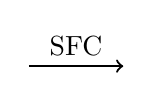
\begin{tikzpicture}[baseline={(current bounding box.center)}, scale=0.4]
            % Arrow from second grid to third grid
            \draw[->, thick] (0, 0) -- (3, 0)
            node[midway, above] {SFC};
        \end{tikzpicture}
        \hspace{2pt} % Decrease space here
        \begin{array}{|p{0.5cm}|p{0.5cm}|p{0.5cm}|p{0.5cm}|}
            \hline
              &   &   &   \\ \hline
            5 & A &   & A \\ \hline
            A & A & D &   \\ \hline
            F &   & 7 & A \\ \hline
        \end{array}
        \hspace{2pt} % Decrease space here
        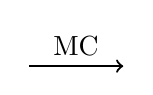
\begin{tikzpicture}[baseline={(current bounding box.center)}, scale=0.4]
            % Arrow from third grid to fourth grid
            \draw[->, thick] (0, 0) -- (3, 0)
            node[midway, above] {MC};
        \end{tikzpicture}
        \hspace{2pt} % Decrease space here
        \begin{array}{|p{0.5cm}|p{0.5cm}|p{0.5cm}|p{0.5cm}|}
            \hline
              &   & A &   \\ \hline
            5 & A & A & A \\ \hline
            A & A &   &   \\ \hline
            F &   & D & A \\ \hline
        \end{array}
        \)
        \hspace{2pt} % Decrease space here
        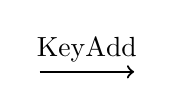
\begin{tikzpicture}[baseline={(current bounding box.center)}, scale=0.4]
            % Arrow from third grid to fourth grid
            \draw[->, thick] (0, 0) -- (3, 0)
            node[midway, above] {KeyAdd};
        \end{tikzpicture}

    }
\end{center}
\begin{center}
    \resizebox{\textwidth}{!}{%
        \(
        \begin{array}{|p{0.5cm}|p{0.5cm}|p{0.5cm}|p{0.5cm}|}
            \hline
              &   & A &   \\ \hline
            5 & A & A & A \\ \hline
            A & A & 7 &   \\ \hline
            F &   & D & A \\ \hline
        \end{array}
        \hspace{2pt} % Decrease space here
        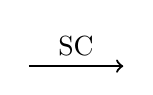
\begin{tikzpicture}[baseline={(current bounding box.center)}, scale=0.4]
            % Arrow from first grid to second grid
            \draw[->, thick] (0, 0) -- (3, 0)
            node[midway, above] {SC};
        \end{tikzpicture}
        \hspace{2pt} % Decrease space here
        \begin{array}{|p{0.5cm}|p{0.5cm}|p{0.5cm}|p{0.5cm}|}
            \hline
              &   & 5 &   \\ \hline
            7 & 5 & A & 5 \\ \hline
            5 & A & 5 &   \\ \hline
            A &   & 7 & 5 \\ \hline
        \end{array}
        \hspace{2pt} % Decrease space here
        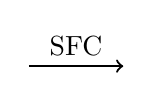
\begin{tikzpicture}[baseline={(current bounding box.center)}, scale=0.4]
            % Arrow from second grid to third grid
            \draw[->, thick] (0, 0) -- (3, 0)
            node[midway, above] {SFC};
        \end{tikzpicture}
        \hspace{2pt} % Decrease space here
        \begin{array}{|p{0.5cm}|p{0.5cm}|p{0.5cm}|p{0.5cm}|}
            \hline
              & A &   &   \\ \hline
            5 &   & A & 5 \\ \hline
            5 & 7 &   & 5 \\ \hline
            5 & 7 & A & 5 \\ \hline
        \end{array}
        \hspace{2pt} % Decrease space here
        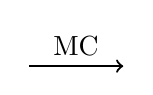
\begin{tikzpicture}[baseline={(current bounding box.center)}, scale=0.4]
            % Arrow from third grid to fourth grid
            \draw[->, thick] (0, 0) -- (3, 0)
            node[midway, above] {MC};
        \end{tikzpicture}
        \hspace{2pt} % Decrease space here
        \begin{array}{|p{0.5cm}|p{0.5cm}|p{0.5cm}|p{0.5cm}|}
            \hline
            5 &   &   & 5 \\ \hline
              &   &   &   \\ \hline
              & 7 & A &   \\ \hline
              & 7 &   &   \\ \hline
        \end{array}
        \)
        \hspace{2pt} % Decrease space here
        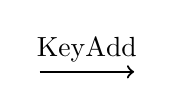
\begin{tikzpicture}[baseline={(current bounding box.center)}, scale=0.4]
            % Arrow from third grid to fourth grid
            \draw[->, thick] (0, 0) -- (3, 0)
            node[midway, above] {KeyAdd};
        \end{tikzpicture}
    }
\end{center}
\begin{center}
    \resizebox{\textwidth}{!}{%
        \(
        \begin{array}{|p{0.5cm}|p{0.5cm}|p{0.5cm}|p{0.5cm}|}
            \hline
            5 &   &   & 5 \\ \hline
              &   &   &   \\ \hline
              & 7 & A &   \\ \hline
              & 7 &   &   \\ \hline
        \end{array}
        \hspace{2pt} % Decrease space here
        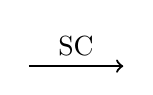
\begin{tikzpicture}[baseline={(current bounding box.center)}, scale=0.4]
            % Arrow from first grid to second grid
            \draw[->, thick] (0, 0) -- (3, 0)
            node[midway, above] {SC};
        \end{tikzpicture}
        \hspace{2pt} % Decrease space here
        \begin{array}{|p{0.5cm}|p{0.5cm}|p{0.5cm}|p{0.5cm}|}
            \hline
            A &   &   & A \\ \hline
              &   &   &   \\ \hline
              & 5 & A &   \\ \hline
              & 5 &   &   \\ \hline
        \end{array}
        \hspace{2pt} % Decrease space here
        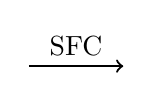
\begin{tikzpicture}[baseline={(current bounding box.center)}, scale=0.4]
            % Arrow from second grid to third grid
            \draw[->, thick] (0, 0) -- (3, 0)
            node[midway, above] {SFC};
        \end{tikzpicture}
        \hspace{2pt} % Decrease space here
        \begin{array}{|p{0.5cm}|p{0.5cm}|p{0.5cm}|p{0.5cm}|}
            \hline
            A &  &   & 5 \\ \hline
            A &  &   &   \\ \hline
              &  & A &   \\ \hline
              &  & 5 &   \\ \hline
        \end{array}
        \hspace{2pt} % Decrease space here
        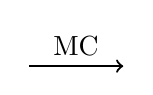
\begin{tikzpicture}[baseline={(current bounding box.center)}, scale=0.4]
            % Arrow from third grid to fourth grid
            \draw[->, thick] (0, 0) -- (3, 0)
            node[midway, above] {MC};
        \end{tikzpicture}
        \hspace{2pt} % Decrease space here
        \begin{array}{|p{0.5cm}|p{0.5cm}|p{0.5cm}|p{0.5cm}|}
            \hline
            A &  & F &   \\ \hline
            A &  & F & 5 \\ \hline
              &  & 5 & 5 \\ \hline
              &  & A & 5 \\ \hline
        \end{array}
        \hspace{2pt} % Decrease space here
        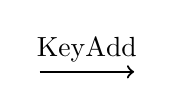
\begin{tikzpicture}[baseline={(current bounding box.center)}, scale=0.4]
            % Arrow from third grid to fourth grid
            \draw[->, thick] (0, 0) -- (3, 0)
            node[midway, above] {KeyAdd};
        \end{tikzpicture}
        \hspace{2pt} % Decrease space here
        \begin{array}{|p{0.5cm}|p{0.5cm}|p{0.5cm}|p{0.5cm}|}
            \hline
            A &  & F &   \\ \hline
            A &  & F & 5 \\ \hline
              &  & 5 & 5 \\ \hline
              &  & A & 5 \\ \hline
        \end{array}
        \)
    }

\end{center}


    where $\delta \in \{5, A, D, F\}$
    \newline

    % %======================================================================================================

    %  fig 1 differential attack
    \text{FIGURE 2. Another 5-round differential path with probability of $2^{-52}$}

\renewcommand{\arraystretch}{1.5} % Adjust the row height
\setlength{\tabcolsep}{0pt} % Remove extra padding between columns
\begin{center}
    \resizebox{\textwidth}{!}{%
        \(

        \begin{array}{|p{0.5cm}|p{0.5cm}|p{0.5cm}|p{0.5cm}|}
            \hline
            \alpha &  &       & \\ \hline
                   &  &       & \\ \hline
                   &  & \beta & \\ \hline
                   &  &       & \\ \hline
        \end{array}
        \hspace{2pt} % Decrease space here
        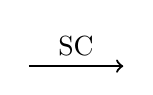
\begin{tikzpicture}[baseline={(current bounding box.center)}, scale=0.4]
            % Arrow from first grid to second grid
            \draw[->, thick] (0, 0) -- (3, 0)
            node[midway, above] {SC};
        \end{tikzpicture}
        \hspace{2pt} % Decrease space here

        \begin{array}{|p{0.5cm}|p{0.5cm}|p{0.5cm}|p{0.5cm}|}
            \hline
            2 &  &   & \\ \hline
              &  &   & \\ \hline
              &  & 2 & \\ \hline
              &  &   & \\ \hline
        \end{array}
        \hspace{2pt} % Decrease space here
        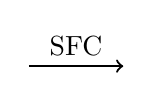
\begin{tikzpicture}[baseline={(current bounding box.center)}, scale=0.4]
            % Arrow from second grid to third grid
            \draw[->, thick] (0, 0) -- (3, 0)
            node[midway, above] {SFC};
        \end{tikzpicture}
        \hspace{2pt} % Decrease space here

        \begin{array}{|p{0.5cm}|p{0.5cm}|p{0.5cm}|p{0.5cm}|}
            \hline
            2 &  &  & \\ \hline
            2 &  &  & \\ \hline
              &  &  & \\ \hline
              &  &  & \\ \hline
        \end{array}
        \hspace{2pt} % Decrease space here
        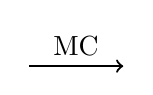
\begin{tikzpicture}[baseline={(current bounding box.center)}, scale=0.4]
            % Arrow from third grid to fourth grid
            \draw[->, thick] (0, 0) -- (3, 0)
            node[midway, above] {MC};
        \end{tikzpicture}
        \hspace{2pt} % Decrease space here
        \begin{array}{|p{0.5cm}|p{0.5cm}|p{0.5cm}|p{0.5cm}|}
            \hline
            2 &  &  & \\ \hline
            2 &  &  & \\ \hline
              &  &  & \\ \hline
              &  &  & \\ \hline
        \end{array}
        \)
        \hspace{2pt} % Decrease space here

        \begin{tikzpicture}[baseline={(current bounding box.center)}, scale=0.4]
            % Arrow from third grid to fourth grid
            \draw[->, thick] (0, 0) -- (3, 0)
            node[midway, above] {KeyAdd};
        \end{tikzpicture}

    }
\end{center}
\begin{center}
    \resizebox{\textwidth}{!}{%
        \(
        \begin{array}{|p{0.5cm}|p{0.5cm}|p{0.5cm}|p{0.5cm}|}
            \hline
            2 &  &  & \\ \hline
            2 &  &  & \\ \hline
              &  &  & \\ \hline
              &  &  & \\ \hline
        \end{array}
        \hspace{2pt} % Decrease space here
        \begin{tikzpicture}[baseline={(current bounding box.center)}, scale=0.4]
            % Arrow from first grid to second grid
            \draw[->, thick] (0, 0) -- (3, 0)
            node[midway, above] {SC};
        \end{tikzpicture}
        \hspace{2pt} % Decrease space here
        \begin{array}{|p{0.5cm}|p{0.5cm}|p{0.5cm}|p{0.5cm}|}
            \hline
            4 &  &  & \\ \hline
            1 &  &  & \\ \hline
              &  &  & \\ \hline
              &  &  & \\ \hline
        \end{array}
        \hspace{2pt} % Decrease space here
        \begin{tikzpicture}[baseline={(current bounding box.center)}, scale=0.4]
            % Arrow from second grid to third grid
            \draw[->, thick] (0, 0) -- (3, 0)
            node[midway, above] {SFC};
        \end{tikzpicture}
        \hspace{2pt} % Decrease space here
        \begin{array}{|p{0.5cm}|p{0.5cm}|p{0.5cm}|p{0.5cm}|}
            \hline
            4 &   &  & \\ \hline
              &   &  & \\ \hline
              &   &  & \\ \hline
              & 1 &  & \\ \hline
        \end{array}
        \hspace{2pt} % Decrease space here
        \begin{tikzpicture}[baseline={(current bounding box.center)}, scale=0.4]
            % Arrow from third grid to fourth grid
            \draw[->, thick] (0, 0) -- (3, 0)
            node[midway, above] {MC};
        \end{tikzpicture}
        \hspace{2pt} % Decrease space here
        \begin{array}{|p{0.5cm}|p{0.5cm}|p{0.5cm}|p{0.5cm}|}
            \hline
              & 1 &  & \\ \hline
            4 & 1 &  & \\ \hline
            4 & 1 &  & \\ \hline
            4 &   &  & \\ \hline
        \end{array}
        \)
        \hspace{2pt} % Decrease space here
        \begin{tikzpicture}[baseline={(current bounding box.center)}, scale=0.4]
            % Arrow from third grid to fourth grid
            \draw[->, thick] (0, 0) -- (3, 0)
            node[midway, above] {KeyAdd};
        \end{tikzpicture}

    }
\end{center}
\begin{center}
    \resizebox{\textwidth}{!}{%
        \(
        \begin{array}{|p{0.5cm}|p{0.5cm}|p{0.5cm}|p{0.5cm}|}
            \hline
              & 1 &  & \\ \hline
            4 & 1 &  & \\ \hline
            4 & 1 &  & \\ \hline
            4 &   &  & \\ \hline
        \end{array}
        \hspace{2pt} % Decrease space here
        \begin{tikzpicture}[baseline={(current bounding box.center)}, scale=0.4]
            % Arrow from first grid to second grid
            \draw[->, thick] (0, 0) -- (3, 0)
            node[midway, above] {SC};
        \end{tikzpicture}
        \hspace{2pt} % Decrease space here
        \begin{array}{|p{0.5cm}|p{0.5cm}|p{0.5cm}|p{0.5cm}|}
            \hline
              & 2 &  & \\ \hline
            2 & 2 &  & \\ \hline
            2 & 2 &  & \\ \hline
            2 &   &  & \\ \hline
        \end{array}
        \hspace{2pt} % Decrease space here
        \begin{tikzpicture}[baseline={(current bounding box.center)}, scale=0.4]
            % Arrow from second grid to third grid
            \draw[->, thick] (0, 0) -- (3, 0)
            node[midway, above] {SFC};
        \end{tikzpicture}
        \hspace{2pt} % Decrease space here
        \begin{array}{|p{0.5cm}|p{0.5cm}|p{0.5cm}|p{0.5cm}|}
            \hline
              &   &   &   \\ \hline
              & 2 & 2 &   \\ \hline
            2 &   &   & 2 \\ \hline
              & 2 & 2 &   \\ \hline
        \end{array}
        \hspace{2pt} % Decrease space here
        \begin{tikzpicture}[baseline={(current bounding box.center)}, scale=0.4]
            % Arrow from third grid to fourth grid
            \draw[->, thick] (0, 0) -- (3, 0)
            node[midway, above] {MC};
        \end{tikzpicture}
        \hspace{2pt} % Decrease space here
        \begin{array}{|p{0.5cm}|p{0.5cm}|p{0.5cm}|p{0.5cm}|}
            \hline
            2 &   &   & 2 \\ \hline
            2 & 2 & 2 & 2 \\ \hline
              &   &   &   \\ \hline
            2 & 2 & 2 & 2 \\ \hline
        \end{array}
        \)
        \hspace{2pt} % Decrease space here
        \begin{tikzpicture}[baseline={(current bounding box.center)}, scale=0.4]
            % Arrow from third grid to fourth grid
            \draw[->, thick] (0, 0) -- (3, 0)
            node[midway, above] {KeyAdd};
        \end{tikzpicture}

    }
\end{center}
\begin{center}
    \resizebox{\textwidth}{!}{%
        \(
        \begin{array}{|p{0.5cm}|p{0.5cm}|p{0.5cm}|p{0.5cm}|}
            \hline
            2 &   &   & 2 \\ \hline
            2 & 2 & 2 & 2 \\ \hline
              &   &   &   \\ \hline
            2 & 2 & 2 & 2 \\ \hline
        \end{array}
        \hspace{2pt} % Decrease space here
        \begin{tikzpicture}[baseline={(current bounding box.center)}, scale=0.4]
            % Arrow from first grid to second grid
            \draw[->, thick] (0, 0) -- (3, 0)
            node[midway, above] {SC};
        \end{tikzpicture}
        \hspace{2pt} % Decrease space here
        \begin{array}{|p{0.5cm}|p{0.5cm}|p{0.5cm}|p{0.5cm}|}
            \hline
            4 &   &   & 1 \\ \hline
            1 & 4 & 1 & 1 \\ \hline
              &   &   &   \\ \hline
            1 & 1 & 1 & 4 \\ \hline
        \end{array}
        \hspace{2pt} % Decrease space here
        \begin{tikzpicture}[baseline={(current bounding box.center)}, scale=0.4]
            % Arrow from second grid to third grid
            \draw[->, thick] (0, 0) -- (3, 0)
            node[midway, above] {SFC};
        \end{tikzpicture}
        \hspace{2pt} % Decrease space here
        \begin{array}{|p{0.5cm}|p{0.5cm}|p{0.5cm}|p{0.5cm}|}
            \hline
            4 &   & 1 & 1 \\ \hline
              &   & 1 & 1 \\ \hline
            4 & 1 & 1 &   \\ \hline
            4 & 1 &   &   \\ \hline
        \end{array}
        \hspace{2pt} % Decrease space here
        \begin{tikzpicture}[baseline={(current bounding box.center)}, scale=0.4]
            % Arrow from third grid to fourth grid
            \draw[->, thick] (0, 0) -- (3, 0)
            node[midway, above] {MC};
        \end{tikzpicture}
        \hspace{2pt} % Decrease space here
        \begin{array}{|p{0.5cm}|p{0.5cm}|p{0.5cm}|p{0.5cm}|}
            \hline
              &   &   & 1 \\ \hline
            4 &   &   & 1 \\ \hline
              & 1 &   &   \\ \hline
              & 1 & 1 &   \\ \hline
        \end{array}
        \)
        \hspace{2pt} % Decrease space here
        \begin{tikzpicture}[baseline={(current bounding box.center)}, scale=0.4]
            % Arrow from third grid to fourth grid
            \draw[->, thick] (0, 0) -- (3, 0)
            node[midway, above] {KeyAdd};
        \end{tikzpicture}
    }
\end{center}
\begin{center}
    \resizebox{\textwidth}{!}{%
        \(
        \begin{array}{|p{0.5cm}|p{0.5cm}|p{0.5cm}|p{0.5cm}|}
            \hline
              &   &   & 1 \\ \hline
            4 &   &   & 1 \\ \hline
              & 1 &   &   \\ \hline
              & 1 & 1 &   \\ \hline
        \end{array}
        \hspace{2pt} % Decrease space here
        \begin{tikzpicture}[baseline={(current bounding box.center)}, scale=0.4]
            % Arrow from first grid to second grid
            \draw[->, thick] (0, 0) -- (3, 0)
            node[midway, above] {SC};
        \end{tikzpicture}
        \hspace{2pt} % Decrease space here
        \begin{array}{|p{0.5cm}|p{0.5cm}|p{0.5cm}|p{0.5cm}|}
            \hline
              &   &   & 2 \\ \hline
            2 &   &   & 2 \\ \hline
              & 2 &   &   \\ \hline
              & 2 & 2 &   \\ \hline
        \end{array}
        \hspace{2pt} % Decrease space here
        \begin{tikzpicture}[baseline={(current bounding box.center)}, scale=0.4]
            % Arrow from second grid to third grid
            \draw[->, thick] (0, 0) -- (3, 0)
            node[midway, above] {SFC};
        \end{tikzpicture}
        \hspace{2pt} % Decrease space here
        \begin{array}{|p{0.5cm}|p{0.5cm}|p{0.5cm}|p{0.5cm}|}
            \hline
             &   &   & 2 \\ \hline
             &   &   & 2 \\ \hline
             & 2 & 2 &   \\ \hline
             & 2 & 2 &   \\ \hline
        \end{array}
        \hspace{2pt} % Decrease space here
        \begin{tikzpicture}[baseline={(current bounding box.center)}, scale=0.4]
            % Arrow from third grid to fourth grid
            \draw[->, thick] (0, 0) -- (3, 0)
            node[midway, above] {MC};
        \end{tikzpicture}
        \hspace{2pt} % Decrease space here
        \begin{array}{|p{0.5cm}|p{0.5cm}|p{0.5cm}|p{0.5cm}|}
            \hline
             &   &   & 2 \\ \hline
             &   &   & 2 \\ \hline
             & 2 & 2 &   \\ \hline
             & 2 & 2 &   \\ \hline
        \end{array}
        \hspace{2pt} % Decrease space here
        \begin{tikzpicture}[baseline={(current bounding box.center)}, scale=0.4]
            % Arrow from third grid to fourth grid
            \draw[->, thick] (0, 0) -- (3, 0)
            node[midway, above] {KeyAdd};
        \end{tikzpicture}
        \hspace{2pt} % Decrease space here
        \begin{array}{|p{0.5cm}|p{0.5cm}|p{0.5cm}|p{0.5cm}|}
            \hline
             &   &   & 2 \\ \hline
             &   &   & 2 \\ \hline
             & 2 & 2 &   \\ \hline
             & 2 & 2 &   \\ \hline
        \end{array}
        \)
    }
\end{center}

    \subsection{Attack on 11-Round Midori64}

    Using the 5-round differential characteristic

    % (\delta, 0, 0, 0, 0, 0, 0, 0, 0, 0, 0, 0, 0, 0, 0, 0) \to (A, A, 0, 0, 0, 0, 0, 0, F, F, 5, A, 0, 5, 5, 5)
    \begin{center}
        \begin{tikzpicture}[node distance=0.01cm and 0cm]
            \node[minimum width=6cm, align=center] (tuple1)
            {(\(\delta, 0, 0, 0, 0, 0, 0, 0, 0, 0, 0, 0, 0, 0, 0, 0\))};
            \node[below=of tuple1, align=center] (arrow) {\(\downarrow\)};
            \node[minimum width=6cm, below=of arrow, align=center] (tuple2)
            {(\(A, A, 0, 0, 0, 0, 0, 0, F, F, 5, A, 0, 5, 5, 5\))};
        \end{tikzpicture}
    \end{center}
    with the probability of $2^{-58}$ in Table 1 and Figure 1, we could launch a key-recovery attack against the 11-round Midori64. We choose the differential-2 rather than the differential-1 because the former is more effective.

    Then, add three rounds at its beginning and the end, respectively, to attack the 11-round reduced Midori64, as shown in Figure 2. The attack procedures are as follows:

    \subsubsection{Data Collection}
    Since the differences of plaintexts are all uncertain bits, plaintexts cannot be classified by inactive bits. Choose any $2^n$ plaintexts and form approximately $2^{2n-1}$ plaintext pairs. Encrypt these plaintext pairs to state $W_1$ and use the difference $\Delta W_1\{0, 1, 2, 3\} = \{0, \ast, \ast, \ast\}$ to filter pairs. By Property 1, this provides a filtering probability of $2^{-4.28}$, and there are approximately $2^{2n-5.28}$ pairs left. Similarly, keep only the pairs such that $\Delta W_1 \{4, 5, 6, 7\} = \{0, 0, \ast, \ast \}, \Delta W_1 \{8, 9, 10, 11\} = \{0, \ast, 0, \ast \}$ and $\Delta W_1 \{12, 13, 14, 15\} = \{0, \ast, \ast, 0\}$. By Property 3, the probability of these three cases is $2^{-8}$ and there are $2^{2n - 29.28}$ pairs left. Therefore, in the data collection phase, the remaining number jof the plaintext/cipertext paires is approximately $2^{2n - 29.28}$ only by the path choosing without guessing the key.
    \newpage
% % 11 round differential 
% %==============================================================================================
\renewcommand{\arraystretch}{1.5} % Adjust the row height
\setlength{\tabcolsep}{0pt} % Remove extra padding between columns

\caption{ 11 round differential}
\begin{center}
    \resizebox{\textwidth}{!}{%
        \(
        \begin{array}{|p{0.5cm}|p{0.5cm}|p{0.5cm}|p{0.5cm}|}
            \hline
            ?    & ?    & ?    & ?    \\ \hline
            \ast & ?    & ?    & \ast \\ \hline
            \ast & \ast & ?    & ?    \\ \hline
            \ast & ?    & \ast & ?    \\ \hline
        \end{array}
        \hspace{2pt} % Decrease space here
        \begin{tikzpicture}[baseline={(current bounding box.center)}, scale=0.4]
            % Arrow from first grid to second grid
            \draw[->, thick] (0, 0) -- (3, 0)
            node[midway, above] {SC};
        \end{tikzpicture}
        \hspace{2pt} % Decrease space here
        \begin{array}{|p{0.5cm}|p{0.5cm}|p{0.5cm}|p{0.5cm}|}
            \hline
            ?    & ?    & ?    & ?    \\ \hline
            \ast & ?    & ?    & \ast \\ \hline
            \ast & \ast & ?    & ?    \\ \hline
            \ast & ?    & \ast & ?    \\ \hline
        \end{array}
        \hspace{2pt} % Decrease space here
        \begin{tikzpicture}[baseline={(current bounding box.center)}, scale=0.4]
            % Arrow from second grid to third grid
            \draw[->, thick] (0, 0) -- (3, 0)
            node[midway, above] {SFC};
        \end{tikzpicture}
        \hspace{2pt} % Decrease space here
        \begin{array}{|p{0.5cm}|p{0.5cm}|p{0.5cm}|p{0.5cm}|}
            \hline
            ? & ?    & ?    & ?    \\ \hline
            ? & ?    & \ast & \ast \\ \hline
            ? & \ast & ?    & \ast \\ \hline
            ? & \ast & \ast & ?    \\ \hline
        \end{array}
        \hspace{2pt} % Decrease space here
        \begin{tikzpicture}[baseline={(current bounding box.center)}, scale=0.4]
            % Arrow from third grid to fourth grid
            \draw[->, thick] (0, 0) -- (3, 0)
            node[midway, above] {MC};
        \end{tikzpicture}
        \hspace{2pt} % Decrease space here
        \begin{array}{|p{0.5cm}|p{0.5cm}|p{0.5cm}|p{0.5cm}|}
            \hline
                 &      &      &      \\ \hline
            \ast &      & \ast & \ast \\ \hline
            \ast & \ast &      & \ast \\ \hline
            \ast & \ast & \ast &      \\ \hline
        \end{array}
        \)
        \hspace{2pt} % Decrease space here

        \begin{tikzpicture}[baseline={(current bounding box.center)}, scale=0.4]
            % Arrow from third grid to fourth grid
            \draw[->, thick] (0, 0) -- (3, 0)
            node[midway, above] {KeyAdd};
        \end{tikzpicture}

    }
\end{center}
\begin{center}
    \resizebox{\textwidth}{!}{%
        \(
        \begin{array}{|p{0.5cm}|p{0.5cm}|p{0.5cm}|p{0.5cm}|}
            \hline
                 &      &      &      \\ \hline
            \ast &      & \ast & \ast \\ \hline
            \ast & \ast &      & \ast \\ \hline
            \ast & \ast & \ast &      \\ \hline
        \end{array}
        \hspace{2pt} % Decrease space here
        \begin{tikzpicture}[baseline={(current bounding box.center)}, scale=0.4]
            % Arrow from first grid to second grid
            \draw[->, thick] (0, 0) -- (3, 0)
            node[midway, above] {SC};
        \end{tikzpicture}
        \hspace{2pt} % Decrease space here
        \begin{array}{|p{0.5cm}|p{0.5cm}|p{0.5cm}|p{0.5cm}|}
            \hline
                     &          &          &          \\ \hline
            \Delta_1 &          & \Delta_2 & \Delta_3 \\ \hline
            \Delta_3 & \Delta_2 &          & \Delta_1 \\ \hline
            \Delta_2 & \Delta_3 & \Delta_1 &          \\ \hline
        \end{array}
        \hspace{2pt} % Decrease space here
        \begin{tikzpicture}[baseline={(current bounding box.center)}, scale=0.4]
            % Arrow from second grid to third grid
            \draw[->, thick] (0, 0) -- (3, 0)
            node[midway, above] {SFC};
        \end{tikzpicture}
        \hspace{2pt} % Decrease space here
        \begin{array}{|p{0.5cm}|p{0.5cm}|p{0.5cm}|p{0.5cm}|}
            \hline
             & \Delta_1 & \Delta_2 & \Delta_3 \\ \hline
             &          & \Delta_2 & \Delta_3 \\ \hline
             & \Delta_1 &          & \Delta_3 \\ \hline
             & \Delta_1 & \Delta_2 &          \\ \hline
        \end{array}
        \hspace{2pt} % Decrease space here
        \begin{tikzpicture}[baseline={(current bounding box.center)}, scale=0.4]
            % Arrow from third grid to fourth grid
            \draw[->, thick] (0, 0) -- (3, 0)
            node[midway, above] {MC};
        \end{tikzpicture}
        \hspace{2pt} % Decrease space here
        \begin{array}{|p{0.5cm}|p{0.5cm}|p{0.5cm}|p{0.5cm}|}
            \hline
             &      &      &      \\ \hline
             & \ast &      &      \\ \hline
             &      & \ast &      \\ \hline
             &      &      & \ast \\ \hline
        \end{array}
        \)
        \hspace{2pt} % Decrease space here
        \begin{tikzpicture}[baseline={(current bounding box.center)}, scale=0.4]
            % Arrow from third grid to fourth grid
            \draw[->, thick] (0, 0) -- (3, 0)
            node[midway, above] {KeyAdd};
        \end{tikzpicture}

    }
\end{center}
\begin{center}
    \resizebox{\textwidth}{!}{%
        \(
        \begin{array}{|p{0.5cm}|p{0.5cm}|p{0.5cm}|p{0.5cm}|}
            \hline
             &      &      &      \\ \hline
             & \ast &      &      \\ \hline
             &      & \ast &      \\ \hline
             &      &      & \ast \\ \hline
        \end{array}
        \hspace{2pt} % Decrease space here
        \begin{tikzpicture}[baseline={(current bounding box.center)}, scale=0.4]
            % Arrow from first grid to second grid
            \draw[->, thick] (0, 0) -- (3, 0)
            node[midway, above] {SC};
        \end{tikzpicture}
        \hspace{2pt} % Decrease space here
        \begin{array}{|p{0.5cm}|p{0.5cm}|p{0.5cm}|p{0.5cm}|}
            \hline
             &        &        &        \\ \hline
             & \delta &        &        \\ \hline
             &        & \delta &        \\ \hline
             &        &        & \delta \\ \hline
        \end{array}
        \hspace{2pt} % Decrease space here
        \begin{tikzpicture}[baseline={(current bounding box.center)}, scale=0.4]
            % Arrow from second grid to third grid
            \draw[->, thick] (0, 0) -- (3, 0)
            node[midway, above] {SFC};
        \end{tikzpicture}
        \hspace{2pt} % Decrease space here
        \begin{array}{|p{0.5cm}|p{0.5cm}|p{0.5cm}|p{0.5cm}|}
            \hline
                   &  &  & \\ \hline
            \delta &  &  & \\ \hline
            \delta &  &  & \\ \hline
            \delta &  &  & \\ \hline
        \end{array}
        \hspace{2pt} % Decrease space here
        \begin{tikzpicture}[baseline={(current bounding box.center)}, scale=0.4]
            % Arrow from third grid to fourth grid
            \draw[->, thick] (0, 0) -- (3, 0)
            node[midway, above] {MC};
        \end{tikzpicture}
        \hspace{2pt} % Decrease space here
        \begin{array}{|p{0.5cm}|p{0.5cm}|p{0.5cm}|p{0.5cm}|}
            \hline
            \delta &  &  & \\ \hline
                   &  &  & \\ \hline
                   &  &  & \\ \hline
                   &  &  & \\ \hline
        \end{array}
        \)
        \hspace{2pt} % Decrease space here
        \begin{tikzpicture}[baseline={(current bounding box.center)}, scale=0.4]
            % Arrow from third grid to fourth grid
            \draw[->, thick] (0, 0) -- (3, 0)
            node[midway, above] {KeyAdd};
        \end{tikzpicture}

    }
\end{center}

%==============================================================begin================================
\(
\begin{array}{|p{0.5cm}|p{0.5cm}|p{0.5cm}|p{0.5cm}|}
    \hline
    \delta &  &  & \\ \hline
           &  &  & \\ \hline
           &  &  & \\ \hline
           &  &  & \\ \hline
\end{array}
\hspace{20pt}
\begin{tikzpicture}[baseline={(current bounding box.center)}, scale=0.6]

    % Arrow to 5-round Differential Characteristic
    \node[draw, thick, minimum height=1.5cm, minimum width=4.5cm, anchor=west] (box) at (0, 0) {5-Round Differential Characteristic};
    \hspace{-10pt}
    \draw[->, thick] (-3, 0) -- (box.west);

    % Outputs: Y_0, Z_0, W_0
    % \node[right=0.5cm of box.east] (Y0) {$Y_0$};
    % \node[right=1.5cm of Y0] (Z0) {$Z_0$};
    % \node[right=1.5cm of Z0] (W0) {$W_0$};

    % Connecting arrows
    % \draw[->, thick] (box.east) -- (Y0.west);

\end{tikzpicture}
\)
% %==============================================================================================
\begin{center}
    \resizebox{\textwidth}{!}{%
        \(
        \begin{array}{|p{0.5cm}|p{0.5cm}|p{0.5cm}|p{0.5cm}|}
            \hline
            A &  & F &   \\ \hline
            A &  & F & 5 \\ \hline
              &  & 5 & 5 \\ \hline
              &  & A & 5 \\ \hline
        \end{array}
        \hspace{2pt} % Decrease space here
        \begin{tikzpicture}[baseline={(current bounding box.center)}, scale=0.4]
            % Arrow from first grid to second grid
            \draw[->, thick] (0, 0) -- (3, 0)
            node[midway, above] {SC};
        \end{tikzpicture}
        \hspace{2pt} % Decrease space here
        \begin{array}{|p{0.5cm}|p{0.5cm}|p{0.5cm}|p{0.5cm}|}
            \hline
            \ast &        & \ast &      \\ \hline
            \ast & \delta & \ast &      \\ \hline
                 &        & \ast & \ast \\ \hline
                 &        & \ast & \ast \\ \hline
        \end{array}
        \hspace{2pt} % Decrease space here
        \begin{tikzpicture}[baseline={(current bounding box.center)}, scale=0.4]
            % Arrow from second grid to third grid
            \draw[->, thick] (0, 0) -- (3, 0)
            node[midway, above] {SFC};
        \end{tikzpicture}
        \hspace{2pt} % Decrease space here
        \begin{array}{|p{0.5cm}|p{0.5cm}|p{0.5cm}|p{0.5cm}|}
            \hline
            \ast & \ast & \ast &      \\ \hline
            \ast &      &      & \ast \\ \hline
                 & \ast & \ast &      \\ \hline
            \ast & \ast &      & \ast \\ \hline
        \end{array}
        \hspace{2pt} % Decrease space here
        \begin{tikzpicture}[baseline={(current bounding box.center)}, scale=0.4]
            % Arrow from third grid to fourth grid
            \draw[->, thick] (0, 0) -- (3, 0)
            node[midway, above] {$MC^{-1}$(K)};
        \end{tikzpicture}
        \hspace{2pt} % Decrease space here
        \begin{array}{|p{0.5cm}|p{0.5cm}|p{0.5cm}|p{0.5cm}|}
            \hline
            \ast & \ast & \ast &      \\ \hline
            \ast &      &      & \ast \\ \hline
                 & \ast & \ast &      \\ \hline
            \ast & \ast &      & \ast \\ \hline
        \end{array}
        \)
        \hspace{2pt} % Decrease space here
        \begin{tikzpicture}[baseline={(current bounding box.center)}, scale=0.4]
            % Arrow from third grid to fourth grid
            \draw[->, thick] (0, 0) -- (3, 0)
            node[midway, above] {MC};
        \end{tikzpicture}

    }
\end{center}

\begin{center}
    \resizebox{\textwidth}{!}{%
        \(
        \begin{array}{|p{0.5cm}|p{0.5cm}|p{0.5cm}|p{0.5cm}|}
            \hline
            ? & ? &      & ?    \\ \hline
            ? & ? & \ast & \ast \\ \hline
            ? & ? & \ast & ?    \\ \hline
            ? & ? & \ast & \ast \\ \hline
        \end{array}
        \hspace{2pt} % Decrease space here
        \begin{tikzpicture}[baseline={(current bounding box.center)}, scale=0.4]
            % Arrow from first grid to second grid
            \draw[->, thick] (0, 0) -- (3, 0)
            node[midway, above] {SC};
        \end{tikzpicture}
        \hspace{2pt} % Decrease space here
        \begin{array}{|p{0.5cm}|p{0.5cm}|p{0.5cm}|p{0.5cm}|}
            \hline
            ? & ? &      & ?    \\ \hline
            ? & ? & \ast & \ast \\ \hline
            ? & ? & \ast & ?    \\ \hline
            ? & ? & \ast & \ast \\ \hline
        \end{array}
        \hspace{2pt} % Decrease space here
        \begin{tikzpicture}[baseline={(current bounding box.center)}, scale=0.4]
            % Arrow from second grid to third grid
            \draw[->, thick] (0, 0) -- (3, 0)
            node[midway, above] {SFC};
        \end{tikzpicture}
        \hspace{2pt} % Decrease space here
        \begin{array}{|p{0.5cm}|p{0.5cm}|p{0.5cm}|p{0.5cm}|}
            \hline
            ?    & ?    & \ast & ?    \\ \hline
            \ast & ?    & ?    & \ast \\ \hline
            ?    & \ast & ?    & ?    \\ \hline
            \ast & ?    & ?    &      \\ \hline
        \end{array}
        \hspace{2pt} % Decrease space here
        \begin{tikzpicture}[baseline={(current bounding box.center)}, scale=0.4]
            % Arrow from third grid to fourth grid
            \draw[->, thick] (0, 0) -- (3, 0)
            node[midway, above] {$MC^{-1}$(K)};
        \end{tikzpicture}
        \hspace{2pt} % Decrease space here
        \begin{array}{|p{0.5cm}|p{0.5cm}|p{0.5cm}|p{0.5cm}|}
            \hline
            ?    & ?    & \ast & ?    \\ \hline
            \ast & ?    & ?    & \ast \\ \hline
            ?    & \ast & ?    & ?    \\ \hline
            \ast & ?    & ?    &      \\ \hline
        \end{array}
        \)
        \hspace{2pt} % Decrease space here
        \begin{tikzpicture}[baseline={(current bounding box.center)}, scale=0.4]
            % Arrow from third grid to fourth grid
            \draw[->, thick] (0, 0) -- (3, 0)
            node[midway, above] {MC};
        \end{tikzpicture}

    }

    \vspace{10pt}
    \resizebox{\textwidth}{!}{%
        \(

        \renewcommand{\arraystretch}{1.5} % Adjust the row height
        \setlength{\tabcolsep}{0pt} % Remove extra padding between columns
        \begin{array}{|p{0.5cm}|p{0.5cm}|p{0.5cm}|p{0.5cm}|} % Fixed column width
            % \begin{array}{|p{0.2cm}|p{0.2cm}|p{0.2cm}|p{0.2cm}|}
            \hline
            ? & ? & ? & ? \\ \hline
            ? & ? & ? & ? \\ \hline
            ? & ? & ? & ? \\ \hline
            ? & ? & ? & ? \\ \hline
        \end{array}
        \hspace{10pt} % Decrease space here
        \begin{tikzpicture}[baseline={(current bounding box.center)}, scale=0.2]
            % Arrow from first grid to second grid
            \draw[->, thick] (0, 0) -- (6, 0)
            node[midway, above] {SC};
        \end{tikzpicture}
        \hspace{10pt} % Decrease space here

        \renewcommand{\arraystretch}{1.5} % Adjust the row height
        \setlength{\tabcolsep}{0pt} % Remove extra padding between columns
        \begin{array}{|p{0.5cm}|p{0.5cm}|p{0.5cm}|p{0.5cm}|} % Fixed column width
            % \begin{array}{|p{0.2cm}|p{0.2cm}|p{0.2cm}|p{0.2cm}|}
            \hline
            ? & ? & ? & ? \\ \hline
            ? & ? & ? & ? \\ \hline
            ? & ? & ? & ? \\ \hline
            ? & ? & ? & ? \\ \hline
        \end{array}
        \hspace{20pt} % Decrease space here
        \begin{tikzpicture}[baseline={(current bounding box.center)}, scale=0.2]
            % Arrow from second grid to third grid
            \draw[->, thick] (0, 0) -- (6, 0)
            node[midway, above] {K};
        \end{tikzpicture}
        \)
    }
\end{center}

    \subsubsection{Key Recovery}

    \begin{enumerate}
        \item \textbf{Guess 12 bits $K_0\{1, 11, 14\} \oplus \alpha_0\{1, 11, 14\}$:}
              Partially encrypt these plaintext pairs. The middle values of the correct pairs should satisfy
              \[
                  \Delta X_2\{1, 4, 11, 14\} = \{\ast, 0, \ast, \ast\}, \quad \Delta Y_2\{1, 4, 11, 14\} = \{\Delta_1, 0, \Delta_1, \Delta_1\}.
              \]
              the pairs can be filtered with a probability of $2^{-7.81}$ (Property 4), leaving approximately $2^{2n-37.09}$ pairs.
              Similarly, guess $K_0\{2, 7, 13\} \oplus \alpha_0\{2, 7, 13\}$, and the correct pairs should satisfy
              \[
                  \Delta Y_2\{2, 7, 8, 13\} = \{\Delta_2, \Delta_2, 0, \Delta_2\}.
              \]
              Then, guess $K_0\{3, 6, 9\} \oplus \alpha_0\{3, 6, 9\}$, and the correct pairs should satisfy
              \[
                  \Delta Y_2\{3, 6, 9, 12\} = \{\Delta_3, \Delta_3, \Delta_3, 0\}.
              \]
              After these steps, there are approximately $2^{2n-52.71}$ pairs left.

        \item \textbf{Guess 12 bits $K_1\{5, 10, 15\} \oplus \alpha_1\{5, 10, 15\}$:}
              For each remaining pair, guess the 12 bits one by one and partially encrypt these pairs. The correct pairs should satisfy
              \[
                  \Delta Y_3\{5, 10, 15\} = \{\delta, \delta, \delta\}, \quad \delta \in \{5, A, D, F\}.
              \]
              This step has a filtering probability of $2^{-7.81} \cdot \frac{4}{15} \approx 2^{-9.72}$ (Property 4), leaving approximately $2^{2n-62.43}$ pairs.

        \item \textbf{Guess $MC^{-1}(K_0 \oplus \alpha_{10})\{0, 4, 5, 8, 10, 12, 15\}$:}
              Decrypt the remaining pairs to state $W_{10}$. Use the following conditions to filter pairs:
              \[
                  \Delta W_{10}\{0, 1, 2, 3\} = \{?, \ast, ?, \ast\}, \quad \Delta W_{10}\{4, 5, 6, 7\} = \{?, ?, \ast, ?\},
              \]
              \[
                  \Delta W_{10}\{8, 9, 10, 11\} = \{\ast, ?, ?, ?\}, \quad \Delta W_{10}\{12, 13, 14, 15\} = \{?, \ast, ?, 0\}.
              \]
              The filtering probabilities are $2^{-0.19}$, $2^{-0.09}$, $2^{-0.09}$ (Property 2), and $2^{-4.09}$ (Property 1), respectively. After this step, there are approximately $2^{2n-66.89}$ pairs left.

        \item \textbf{Guess $MC^{-1}(K_1 \oplus \alpha_9)\{0, 1, 2, 3, 4, 6, 7, 8, 9, 11, 12, 13, 14\}$:}
              Decrypt the remaining pairs to state $W_9$ and apply the following filtering conditions:
              \[
                  \Delta W_9\{0, 1, 2, 3\} = \{\ast, \ast, 0, \ast\}, \quad \Delta W_9\{4, 5, 6, 7\} = \{\ast, 0, \ast, \ast\},
              \]
              \[
                  \Delta W_9\{8, 9, 10, 11\} = \{\ast, 0, 0, 0\}, \quad \Delta W_9\{12, 13, 14, 15\} = \{0, \ast, 0, \ast\}.
              \]
              The filtering probabilities are $2^{-4.28}$, $2^{-4.28}$ (Property 1), $2^{-7.81}$ (Property 4), and $2^{-8}$ (Property 3), respectively. After this step, there are approximately $2^{2n-91.26}$ pairs left.

        \item \textbf{Final Decryption:}
              Decrypt the remaining pairs to state $X_9$. Use the condition
              \[
                  \Delta X_9\{0, 1, 8, 9, 10, 11, 13, 14, 15\} = \{A, A, F, F, 5, A, 5, 5, 5\}
              \]
              to filter pairs one by one. This final step has a total filtering probability of $2^{-35.19}$. After this step, there are approximately $2^{2n-126.45}$ pairs left.
    \end{enumerate}


    \subsubsection{Complexity Analysis}

    \textbf{Data Complexity:}
    To distinguish the correct key from the wrong ones, choose $n = 61.2$. For a random key, there are approximately $2^{2 \times 61.2 - 126.45} \approx 2^{-4.05}$ pairs left. However, for the correct key, there are $2^{2 \times 61.2 - 62.43 - 58} \approx 4$ pairs left as the probability of the 5-round differential Path is $2^{-58}$. Thus, the data complexity is $2^{61.2}$ chosen plaintexts.\\
    \newline
    \textbf{Time Complexity:}
    \begin{enumerate}
        \item There are $2^{2n-29.28} = 2^{93.12}$ pairs left after the phase of data collection.
              Guess 12 bits $K_0\{1, 11, 14\} \oplus \alpha_0\{1, 11, 14\}$, then partially encrypt these plaintext pairs for one round.
              The time complexity is
              \[
                  2^{93.12} \times 2 \times 2^{12} \times \frac{3}{16} \times \frac{1}{11} \approx 2^{100.25}
              \]
              11-round encryptions, and the number of remaining pairs is $2^{85.31}$.

              Similarly, guess $K_0\{2, 7, 13\} \oplus \alpha_0\{2, 7, 13\}$, and the time complexity is
              \[
                  2^{85.31} \times 2 \times 2^{12} \times \frac{3}{16} \times \frac{1}{11} \approx 2^{92.44}
              \]
              11-round encryptions, and the number of remaining pairs is $2^{77.5}$.

              Then, guess $K_0\{3, 6, 9\} \oplus \alpha_0\{3, 6, 9\}$, and the time complexity is
              \[
                  2^{84.63}
              \]
              11-round encryptions, and the number of remaining pairs is $2^{69.69}$.

        \item For every remaining pair, guess 12 bits $K_1\{5, 10, 15\} \oplus \alpha_1\{5, 10, 15\}$, and the time complexity is
              \[
                  2^{69.69} \times 2 \times 2^{12} \times \frac{3}{16} \times \frac{1}{11} \approx 2^{76.82}
              \]
              11-round encryptions, and the number of remaining pairs is $2^{59.97}$.

        \item Guess $MC^{-1}(K_0 \oplus \alpha_{10})\{1, 2, 3, 6, 7, 9, 11, 13, 14\}$, and for the whole round, the time complexity is
              \[
                  2^{59.97} \times 2 \times 2^{28} \times \frac{1}{11} \approx 2^{85.51}
              \]
              11-round encryptions, and the number of remaining pairs is $2^{55.51}$.

        \item Similarly, guess $MC^{-1}(K_1 \oplus \alpha_9)\{1, 6, 8\}$, and the time complexity is
              \[
                  2^{55.51} \times 2 \times 2^{12} \times \frac{3}{16} \times \frac{1}{11} \approx 2^{62.64}
              \]
              11-round encryptions, and the number of remaining pairs is $2^{47.7}$.

              Guess $MC^{-1}(K_1 \oplus \alpha_9)\{3, 4, 13\}$, and the time complexity is
              \[
                  2^{47.7} \times 2 \times 2^{12} \times \frac{4}{16} \times \frac{1}{11} \approx 2^{55.24}
              \]
              11-round encryptions, and the number of remaining pairs is $2^{39.7}$.

              Guess $MC^{-1}(K_1 \oplus \alpha_9)\{0, 7, 9, 14\}$, and the time complexity is
              \[
                  2^{39.7} \times 2 \times 2^{16} \times \frac{4}{16} \times \frac{1}{11} \approx 2^{51.24}
              \]
              11-round encryptions, and the number of remaining pairs is $2^{35.42}$.

              Guess $MC^{-1}(K_1 \oplus \alpha_9)\{2, 11, 12\}$, and the time complexity is
              \[
                  2^{35.42} \times 2 \times 2^{12} \times \frac{3}{16} \times \frac{1}{11} \approx 2^{42.55}
              \]
              11-round encryptions, and the number of remaining pairs is $2^{31.14}$.

        \item Finally, the time complexity is
              \[
                  2^{31.14} \times 2 \times \frac{9}{16} \times \frac{1}{11} \approx 2^{27.85}
              \]
              11-round encryptions.

              Thus, the total time complexity is
              \[
                  2^{100.26}
              \]
              11-round encryptions.
    \end{enumerate}


    \subsection{Complexity Analysis of another differential path with probability of $2^{-52}$}

    Similarly, add 3 rounds at the beginning and at the end of the differential
    path with a probability of $2^{-52}$ to attack the 11-round reduced
    Midori64. It is easy to get the probability of $2^{-56.18}$ for the top 3
    rounds.

    Thus, we choose $n = 55.6$. For a random key, there are approximately
    \[
        2^{2 \times 55.6 - 1 - 56.18 - 64} \approx 2^{-10}
    \]
    pairs left. However, for the correct key, there are
    \[
        2^{2 \times 55.6 - 1 - 56.18 - 52} \approx 4
    \]
    pairs left, as the probability of the 5-round differential path is $2^{-52}$.

    Therefore, the data complexity is $2^{55.6}$ chosen plaintexts, and the time
    complexity is $2^{109.35}$ 11-round encryptions, correspondingly.

\newpage
\section{MILP Model}
\subsection*{Introduction}

The Midori64 block cipher is a lightweight substitution-permutation network
(SPN) cipher, designed with a focus on simplicity and security. The MILP model
for Midori64 aims to study and optimize the differential characteristics of the
cipher. This model captures the linear constraints for the cipher's round
operations, such as the non-linear S-box function, cell shuffling, and column
mixing, to calculate the minimal number of active S-boxes. The model uses the
concept of convex hulls to describe the relationship between the input and
output differences, which simplifies the analysis and computation.

The MILP model can be divided into three primary operations, each described by
its set of constraints.


\subsection{Substitution Cell Operation}

The substitution cell involves a transformation from the input variables \(
x_i^j \) to the output variables \( y_i^j \) through a substitution box (S-box  $a_i^j$ ).
The key components are as follows:

\begin{itemize}
    \item \( x_i^j \): Binary input variables where \( i \) is the round number
          and \( j \) is the variable index (ranging from 0 to 63).
    \item \( a_i^j \): Binary variable indicating whether the S-box \( j \) is
          active in round \( i \).
    \item \( p_i^j_k \): Probability binary variables for each S-box and each
          input-output pair, where \( k \) can take values 0 or 1.
    \item \( y_i^j \): Binary output variables where \( i \) is the round number and \( j \) is the variable index (ranging from 0 to 63).
\end{itemize}

% \begin{center}
% \includegraphics[width=5.5cm]{../images/subcell.png}
% \end{center}

The transformation is done through a set of constraints for each nibble (group
of 4 input/output variables) of the substitution.

\subsection*{Constraints}

For each nibble of input \( x_{i,0}, x_{i,1}, x_{i,2}, x_{i,3} \) and output \( y_{i,0}, y_{i,1}, y_{i,2}, y_{i,3} \), the following constraints are applied:

\begin{align*}
    x_{i,0} - a_{i,0}                                                                  & \leq 0 \\
    x_{i,1} - a_{i,0}                                                                  & \leq 0 \\
    x_{i,2} - a_{i,0}                                                                  & \leq 0 \\
    x_{i,3} - a_{i,0}                                                                  & \leq 0 \\
    x_{i,0} + x_{i,1} + x_{i,2} + x_{i,3} - a_{i,0}                                    & \geq 0 \\
    4(x_{i,0} + x_{i,1} + x_{i,2} + x_{i,3}) - (y_{i,0} + y_{i,1} + y_{i,2} + y_{i,3}) & \geq 0 \\
    4(y_{i,0} + y_{i,1} + y_{i,2} + y_{i,3}) - (x_{i,0} + x_{i,1} + x_{i,2} + x_{i,3}) & \geq 0
\end{align*}


\begin{itemize}
    \item \( \highlightmath{x_{i,j} - a_{i,j} \leq 0} \):
          This constraint ensures that the values of \(x_{i,j}\) do not exceed the threshold represented by \(a_{i,j}\). It limits the possible states of \(x_{i,j}\), preventing values of \(x_{i,j}\) from surpassing the allowable range determined by \(a_{i,j}\).

    \item \(\highlightmath{x_{i,0} + x_{i,1} + x_{i,2} + x_{i,3} - a_{i,0} \geq 0}\):
          This constraint ensures that the sum of the elements in the first nibble of \(x_i\) (i.e., \(x_{i,0}, x_{i,1}, x_{i,2}, x_{i,3}\)) is greater than or equal to the threshold value \(a_{i,0}\). It eliminates combinations where the total value of \(x_i\) is too small, ensuring it meets the minimum threshold.

    \item \(\highlightmath{4(x_{i,0} + x_{i,1} + x_{i,2} + x_{i,3}) - (y_{i,0} + y_{i,1} + y_{i,2} + y_{i,3}) \geq 0}\):
          This constraint ensures that four times the sum of the values in \(x_i\) is always greater than or equal to the sum of the corresponding values in \(y_i\). It removes invalid combinations where the values of \(y_i\) could exceed the scaled value of \(x_i\), maintaining a consistent relationship between the variables.

    \item \(\highlightmath{4(y_{i,0} + y_{i,1} + y_{i,2} + y_{i,3}) - (x_{i,0} + x_{i,1} + x_{i,2} + x_{i,3}) \geq 0}\):
          This constraint does the reverse of the previous one, ensuring that the scaled sum of the values in \(y_i\) is greater than or equal to the sum of the corresponding values in \(x_i\). It eliminates combinations where the \(x_i\) values could overpower the \(y_i\) values, ensuring balance and validity between the two.

\end{itemize}


\subsection*{Differential Distribution Table (DDT) and Convex Hull}

The Differential Distribution Table (DDT) is used to describe the probability
distribution of differences in the output (delta-out) for given differences in
the input (delta-in). This table helps to identify impossible transition from
form input to \texttt{Sbox} and it's output from \texttt{Sbox}.

\subsection*{Convex Hull and its Role}
The concept of a convex hull plays a significant role in optimizing the
inequalities generated by the DDT. A convex hull is the smallest convex set that
contains a set of points, and it helps in defining the feasible region for the
inequalities.

By using the convex hull, we can construct a set of inequalities that represent
the feasible region for the DDT. These inequalities will help in constraining
the possible output patterns, thus making help to find differential possible pattern by
eliminating impossible patterns.

\begin{center}
    \includegraphics[width=10cm]{./images/convex_hull.png}
\end{center}

\subsection*{Constructing Parameters and Inequalities}
\begin{itemize}
    \item We first generate the DDT, which describes how changes in the input affect the output of the S-box.
    \item Next, we identify the possible and impossible points based on the DDT.
          The possible points represent valid input-output pairs with non-zero
          probabilities.
    \item Using the convex hull, we generate inequalities that describe the
          feasible region of the DDT.
    \item Each inequality defines a region of valid patterns that satisfy the
          constraints imposed by the SubCell transformation.
\end{itemize}

\subsection*{Generating 239 Inequalities Using Convex Hull}
To generate all 239 inequalities for the Sigle SBox from transformation, we
first construct a polyhedron using the convex hull of the possible points. Then,
we extract the inequalities from the polyhedron representation. This step
provides a comprehensive set of constraints that define the valid regions of the
DDT.

\begin{align*}
    \text{Convex Hull Constraints:} \quad \sum_{i=1}^{n} \text{coeff}_i \cdot x_i + b \geq 0 \\
    x_i = (x_0,x_1,x_2,x_3,y_0,y_1,y_2,y_3,p_0,p_1)
\end{align*}
and mapping for the $p_i$ to probabilities from DDT is as follows

\begin{center}
    \includegraphics[width=5.5cm]{./images/table.png}
\end{center}

This inequality represents the constraints for each region of the convex hull,
where the coefficients \( \text{coeff}_i \) and the constant \( b \) are derived
from the convex hull construction.

\subsection*{Greedy Algorithm to Reduce Constraints}
Once the convex hull has been constructed, the next step is to reduce the number
of constraints. This is done using a greedy algorithm that selects the most
effective inequalities to keep while discarding redundant ones. The greedy
algorithm iteratively removes inequalities that do not significantly reduce the
feasible region.

The algorithm works by comparing the number of impossible points that each
inequality removes. The best inequality is selected, and the process continues
until a reduced set of constraints is achieved.

The Python code for this process is provided below:

\begin{lstlisting}[language=Python]
def reduce_inequalites(inequalities, impossible_points):
    reduced_set = set()

    while impossible_points:
        best_inequality = None
        max_removed_patterns = 0

        for inequality in inequalities:
            removed_patterns = removed_impossible_patterns(
                inequality, impossible_points)

            if len(removed_patterns) > max_removed_patterns:
                max_removed_patterns = len(removed_patterns)
                best_inequality = inequality

        if best_inequality is not None:
            removed_patterns = removed_impossible_patterns(
                best_inequality, impossible_points)

            impossible_points = [point for point in impossible_points 
                                 if point not in removed_patterns]
            reduced_set.add(best_inequality)
            inequalities.remove(best_inequality)

    return reduced_set
\end{lstlisting}

This code effectively reduces the number of inequalities from 239 to 26 by
selecting the most impactful constraints for Differential Distribution Table (DDT).
These 26 Constraints are as follows:
\begin{center}
    \includegraphics[width=10cm]{./images/sbox_equations.png}
\end{center}

This pattern repeats for all 16 S-boxes (from \( a_0 \) to \( a_{15} \)) in a
single round \( i \).


\subsection{Suffle Cell Operation}

The \textbf{ShuffleCell} operation ensures diffusion by shuffling the input values (\( y_{i,j} \)) into
new positions to produce the output values (\( z_{i,j} \)).

\textbf{Transformation Rules}

\[
    (z_0, z_1, z_2, \ldots, z_{15}) \leftarrow (y_0, y_{10}, y_5, y_{15}, y_{14}, y_{4}, y_{11}, y_{1}, y_{9}, y_{3}, y_{12}, y_{6}, y_{7}, y_{13}, y_{2}, y_{8})
\]

This rule specifies that \( z_k \) is derived from \( y_r \), where the
positions \( k \) and \( r \) are determined by the shuffle operation.

To mathematically express this transformation, we define constraints at the
\textbf{4-bit nibble layer}. Each nibble consists of four binary variables, and
the constraints enforce equality between corresponding input (\( y \)) and
output (\( z \)) values.

For each \( z_k \leftarrow y_r \),:

\[
    y_{i,(4r+0)} - z_{i,(4k+0)} = 0
\]
\[
    y_{i,(4r+1)} - z_{i,(4k+1)} = 0
\]
\[
    y_{i,(4r+2)} - z_{i,(4k+2)} = 0
\]
\[
    y_{i,(4r+3)} - z_{i,(4k+3)} = 0
\]

This pattern repeat for all 16 nibbles.

\subsection{MixColumn Operation}

The MixColumn operation in Midori64 is designed to mix the state values in a
manner that diffuses the bits across the cipher. For each round, the output
state \(w_i\) is derived from the input state \(z_i\) using a matrix
multiplication with a predefined mixing matrix. This is performed column-wise,
which leads to the construction of intermediate variables and the subsequent
inequalities.

The mixing matrix for Midori64 is:

\[
    \begin{bmatrix}
        0 & 1 & 1 & 1 \\
        1 & 0 & 1 & 1 \\
        1 & 1 & 0 & 1 \\
        1 & 1 & 1 & 0
    \end{bmatrix}
\]

The MixColumn operation can be viewed as a bit-level operation in which each column of the matrix produces an output \(w_i\) from the inputs \(z_i\). Specifically, for each column, intermediate variables \(t_i\) are used to simplify the addition of the input bits. The input \(z_i\) and output \(w_i\) bits are constrained as follows:

\[
    w_0 = t_0 + z_{12}, \quad w_1 = t_1 + z_{13}, \quad w_2 = t_2 + z_{14}, \quad w_3 = t_3 + z_{15}
\]

Where the intermediate variables are defined as:

\[
    t_0 = z_4 + z_8, \quad t_1 = z_5 + z_9, \quad t_2 = z_6 + z_{10}, \quad t_3 = z_7 + z_{11}
\]

This allows us to break down the constraints into smaller equations.

\subsubsection*{Variables Constraints}
For the each equality mentioned above we will get 4 inequlity.

For xor operation \( c = a \oplus b \):

\[
    a + b - c \geq 0
\]
\[
    a - b + c \geq 0
\]
\[
    -a + b + c \geq 0
\]
\[
    a + b + c \leq 2
\]

These constraints hold for all \(w_i\), ensuring that each output bit is the
result of the proper sum of the intermediate and input bits. Here we are indroducing
32 intermediate variables and getting 384 inequlities in total.

\subsection{Optimization Function}

The optimization function is maximizing summation of differential probabilities
across all S-boxes for the current round \( i \). Which result in the minimizing the
summation of $p_0,p_1$ for all SBoxes with weights $2,3$

\[
    \text{Optimization Function} = \sum_{i,j}^{} \left( 2p_{i,j,0} + 3p_{i,j,1} \right)
\]
%%%% 8. BILBIOGRAPHY %%%%
\bibliographystyle{alpha}
\bibliography{main}


\end{document}
